\documentclass[11pt]{article}
\usepackage[a4paper, hmargin={2.8cm, 2.8cm}, vmargin={2.5cm, 2.5cm}]{geometry}
\usepackage{eso-pic} % \AddToShipoutPicture
\usepackage{graphicx} % \includegraphics
\graphicspath{{/Users/thomas/Skole/Dropbox/SKOLE/}}
\usepackage{amsmath}
\usepackage{amsfonts}
\usepackage{amssymb}
\usepackage{graphicx}
\usepackage{fancyhdr}
\usepackage{moreverb}
\usepackage{lscape}
\usepackage[utf8]{inputenc}
\usepackage{caption}
\usepackage{subcaption}
\usepackage{float}

% Ved at bruge kommandoen \newcommand kan man forkorte kommandoer eller ændre dem til noget mere passende.
\newcommand{\setR}{\mathbb{R}}
\newcommand{\setZ}{\mathbb{Z}}
\newcommand{\setN}{\mathbb{N}}
\newcommand{\setF}{\mathbb{F}}
\newcommand{\lra}{\Leftrightarrow}
\newcommand{\ra}{\Rightarrow}
\newcommand{\ac}{\textasciicircum}
\newcommand{\uuline}[1]{\underline{\underline{#1}}}
\newcommand{\bpm}{\begin{pmatrix}}
\newcommand{\epm}{\end{pmatrix}}

\renewcommand{\headrulewidth}{0pt}

\author{
  \Large{}
  \\ \texttt{} \\
}

\title{Bachelor navn
  \vspace{3cm}
  \Huge{} \\
  \Large{Thomas Nyegaard-Signori}
}

\begin{document}

%% Change `ku-farve` to `nat-farve` to use SCIENCE's old colors or
%% `natbio-farve` to use SCIENCE's new colors and logo.
\AddToShipoutPicture*{\put(0,0){\includegraphics*[viewport=0 0 700 600]{include/ku-farve}}}
\AddToShipoutPicture*{\put(0,602){\includegraphics*[viewport=0 600 700 1600]{include/ku-farve}}}

%% Change `ku-en` to `nat-en` to use the `Faculty of Science` header
\AddToShipoutPicture*{\put(0,0){\includegraphics*{include/ku-en}}}

\clearpage\maketitle
\thispagestyle{empty}

\newpage

% !TeX root = ../report.tex
\section{Introduction}
We communicate via natural language, but it is not only the message that is communicated, it is also the sentiment and intensity of that sentiment. Intensity of sentiment in sentences and words are borderline subjective and therefore difficult to classify in general. Therefore it is interesting to see if it is possible to build a model or program that can do that automatically. \\
To do this we use Natural Language Processing (NLP), and in this field detecting emotion or sentiment in text can be used for analysing stance towards political statements or online consumer reviews of products. \\
Twitter is a great service for detecting these sentiments, since it is user-written and often emotionally fuelled(spelling?).
\subsection{Task} \label{sec:task}
The task to be solved is the SemEval-2018 Task 1: Affect in Tweets, and can be found on \hyperref[https://competitions.codalab.org/competitions/17333]{https://competitions.codalab.org/competitions/17333}. The task is split into five subtasks:\\
\begin{enumerate}
\item EI-reg (Given a tweet and an emotion E, determine the  intensity of E that best represents the mental state of the tweeter—a real-valued score between 0 (least E) and 1 (most E).)
\item EI-oc (Given a tweet and an emotion E, classify the tweet into one of four ordinal classes of intensity of E that best represents the mental state of the tweeter.)
\item V-reg (Given a tweet, determine the intensity of sentiment or valence (V) that best represents the mental state of the tweeter—a real-valued score between 0 (most negative) and 1 (most positive).)
\item V-oc (Given a tweet, classify it into one of seven ordinal classes, corresponding to various levels of positive and negative sentiment intensity, that best represents the mental state of the tweeter.)
\item E-c (Given a tweet, classify it as 'neutral or no emotion' or as one, or more, of eleven given emotions that best represent the mental state of the tweeter.)
\end{enumerate}
 
For all of these subtasks, three language subsubtasks are present, for english, spanish and arabic.\\ 
\subsection{Models}
To best solve these subtasks we use different models to compare and analyse which are better for each subtask. Furthermore we try 2 different approaches to solve the tasks. One approach is the feature based approach which builds on the bag-of-words model (En reference måske?), which takes into account the individual words but not the context in which the words are placed in the sentence. The other approach is the Deep Learning(igen reference måske?) way, in which we implement a variation of a Recurrent Neural Network (RNN), called a gated recurrent unit.

% !TeX root = ../report.tex

\section{Related work}

\subsection{Sentiment analysis}

Semantic analysis and Twitter have been combined before. The SemEval tasks this report and models attempt to solve have been tried before. A lot of different approaches and general task overview has been outlined in \cite{wassa2017}, which is written by the creators of the task.\\
The winning team of the SemEval EmoInt 2017, Prayas, have tackled a similar task as the regression task (task 1, in this report). The winning system utilized an ensemble approach consisting of 5 sub models and using a weighted average of these models to come up with the final result \cite{prayas}. This model is utilizing most of the different approaches mentioned in the literature and combining them into one and with great success. The model presented in this report will test out a simpler method and the influence of different hyperparameters and their direct correlation with the output scores of the model.\\
The runner up in the SemEval EmoInt 2017, \cite{ims}, used a comparatively simpler model consisting of a CNN-LSTM neural network which bears resemblance to the model presented in this report. The difference between the models presented in this report and the IMS system is the utilization of lexicons and training their model on singular emotions (anger, fear, joy or sadness).\\

\subsection{SemEval tasks}
The main task solved in this report is one of many different tasks presented by SemEval-2018. Affect is only one of multiple fields of interest. Coreference, information retrieval, lexical semantics and more are all represented. One of the shared task in the same field as the one being solved in this report is that of multilingual emoji prediction. Another one is a task of irony detection. Both of these are closely related, in that they operate on tweets but also with regards to sentiment detection. 

% !TeX root = ../report.tex

\section{Feature based approach}\label{sec:feature}

For the feature based approach, a feature extraction is done with regards to the term frequency - inverse document frequency. This has been the golden standard for feature extraction, and ensures that the features extracted have the highest descriptive effect with regards to the tweets in which the feature occurs versus the tweets in which the feature does not. These extracted features are then used for the training of one of two different models, depending on the subtask at hand.\\
Both models builds on the random forest learning method since its properties supports both regression and multi-label classification. \\
The two models share the same general feature extraction, so they can be made directly comparable if the extraction parameters are kept comparatively the same.

\subsection{Custom features}
Besides the Tf-idf feature extraction method, we have implemented our own custom feature extraction function. In this function we have different flags, corresponding to different features that could be of interest in these particular tweets. \\
These different custom features involves e.g. whether or not a hashtag is present or if the spelling error of the whole tweet is above some threshold set by us. All of these custom features are boolean values in the sense that they are either present or not. \\
These features are then appended to the feature matrix returned by the Tf-idf extraction function, so that they are taken into consideration when training the different models. \\
Custom features can be based on linguistic and contextual intuition as well as a higher degree of linguistic analysis, as opposed to the deep learning features which will be trained with a more mathematically and statistical paradigm in mind.

\subsection{Model overview}
All the models share the same feature extraction method and the actual models were implemented using libraries which allowed a very high level approach. This acted as an introduction to the subtasks and which ones would be interesting to focus on and also as a baseline system which would work as a stepstone for the deep learning models used later in the process. In the final version of the code, two feature based models were used:\\
\begin{itemize}
 \item Random forest classifier
 \item Random forest regressor
\end{itemize}

\subsection{Results and data}
davdav

% !TeX root = ../report.tex

\section{Deep Learning} \label{sec:deep}
In this section, an overview of the model used in the "deep learning" attempt at solving task 1 and 5 will be presented. The model seeks to solve two subtasks in one go as a multitask learning problem. The subtasks are: regression (task 1 in section \ref{sec:task}) and classification (task 5 in section \ref{sec:task}). For task 1 the model also predicts independently of the general emotion felt, i.e. tweets for joy, anger etc. get a 0-to-1 score using the same model. \\
The multitask model itself a hard parameter sharing model, meaning the weights of the model is shared between the main and auxiliary task being solved, and the model itself is built in Keras, the Python based neural network wrapper for Tensorflow. 

\subsection{Model overview}

\subsubsection{Preprocessing of text and textual representation} \label{sec:preprop}
For the textual preprocessing, all tweets are read in and converted using a mapping from a word to an integer. This ensures that similar words get mapped to the same key and also enables an enforcing on the maximum amount of words to be used. Train data is treated differently than development and test data, in that every unique word read in train data gets converted to the word vector associated with the word. If an unknown word gets read in the development or test data its numerical value gets replaced by an "unknown" placeholder. One way of countering this is to use pretrained word embeddings. This does not constitute as having read and adapted to the test set, since one could envision having a pretrained word embedding for every word in the entire language. Furthermore, user mentions and numbers get mapped to a placeholder value instead of reading in their actual values.\\
The embedding weights used in the model are retrieved from a large set of pretrained embeddings which have been trained on Twitter data ($\sim$400 million tweets). The model used is created by the authors of \cite{godin}. The words in the dataset for the task at hand are then looked up in the pretrained embeddings. If these are not present a zero vector is used instead, which will then be trained from the ground up by the model.\\
Since the model used both word and character representations, the characters were read in separately, although the same basic principle was followed. Every character had a integer mapped to them and this integer would then map to a high dimensional vector with weights that could then be optimized by the network. No pretrained embeddings were used for the characters and so they had to be trained from the ground up, every time.

\subsubsection{Augmentation of data} \label{sec:augm}
The first iteration of the data augmentation consisted of reading in all the data for task 1 and 5 as described in section \ref{sec:preprop}. Since the tweets had different formats of truth labels, one was a singular value (regression) and one was a multi-label list (classification), reading in the labels had to be augmented. Since the tweets were reused in the two tasks, some of the regression tweets could be augmented with their respective classification label, although, if no classification label was present the truth labels were set to -1, which would then act as a mask. Since there were more regression tweets than classification, the augmentation was done this way around.\\
All the tweet representations were padded differently based on whether or not the tweet was being read as a word representation or character representation, and tweets longer than the specified padding values were cut down to size. 

\subsubsection{Word input model}
The word input to the model are 60  $\cdot$ 400 dimensional vectors that have been passed through the preprocessing and augmentation specified in section \ref{sec:preprop} and \ref{sec:augm}. These vectors are then passed into two 250-dimensional, bidirectional GRUs which traverse the tweet front to back and vice versa, and the outputs of the two GRU layers are then concatenated. This output is then batch normalized and a dropout is applied. This output of the word submodel is then concatenated later with the character submodel\\
\begin{figure}[H]
	\centering
		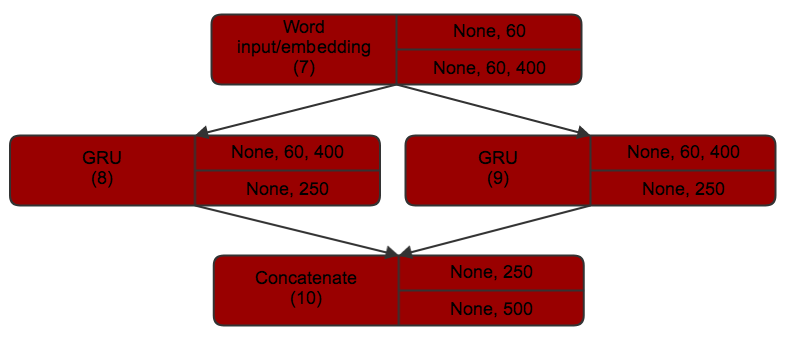
\includegraphics[scale=0.25]{pictures/word_model.png}
		\caption{The word input part of the full model}
		\label{fig:wordmodel}
\end{figure}
\subsubsection{Character input model}
The character input to the model are 256 $\cdot$ 400 dimensional vectors that have been through the same preprocessing and augmentation as the word inputs. These vectors then furthermore get passed into a residual neural network which works as a loop of batch normalizations, dropout applications and 1-dimension convolutions. Each loop ends with an layer-addition of the previous loop layer with the current loop layer and then a max pooling. These vectors are then passed into two GRU layers similar to the word input which are then concatenated and passed along to be connected with the word input part.
\begin{figure}[H]
	\centering
		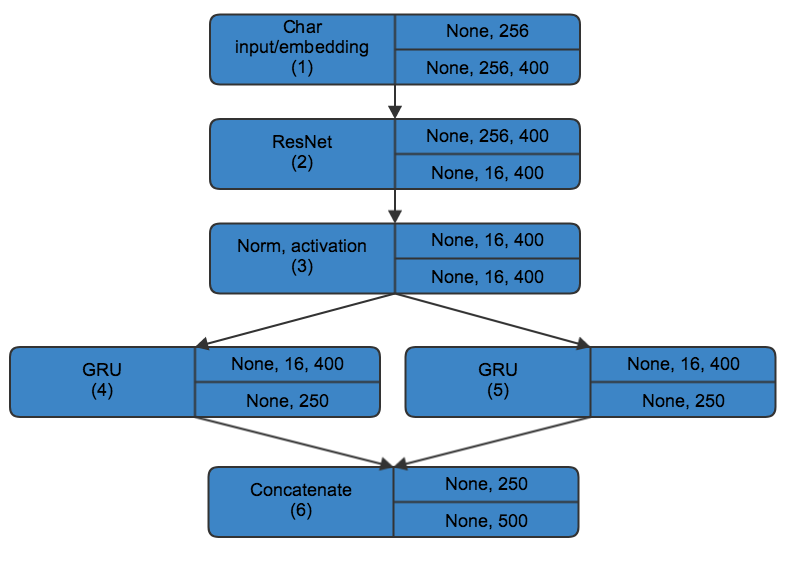
\includegraphics[scale=0.25]{pictures/char_model.png}
		\caption{The character input part of the full model}
		\label{fig:charmodel}
\end{figure}
\begin{figure}[H]
    \centering
        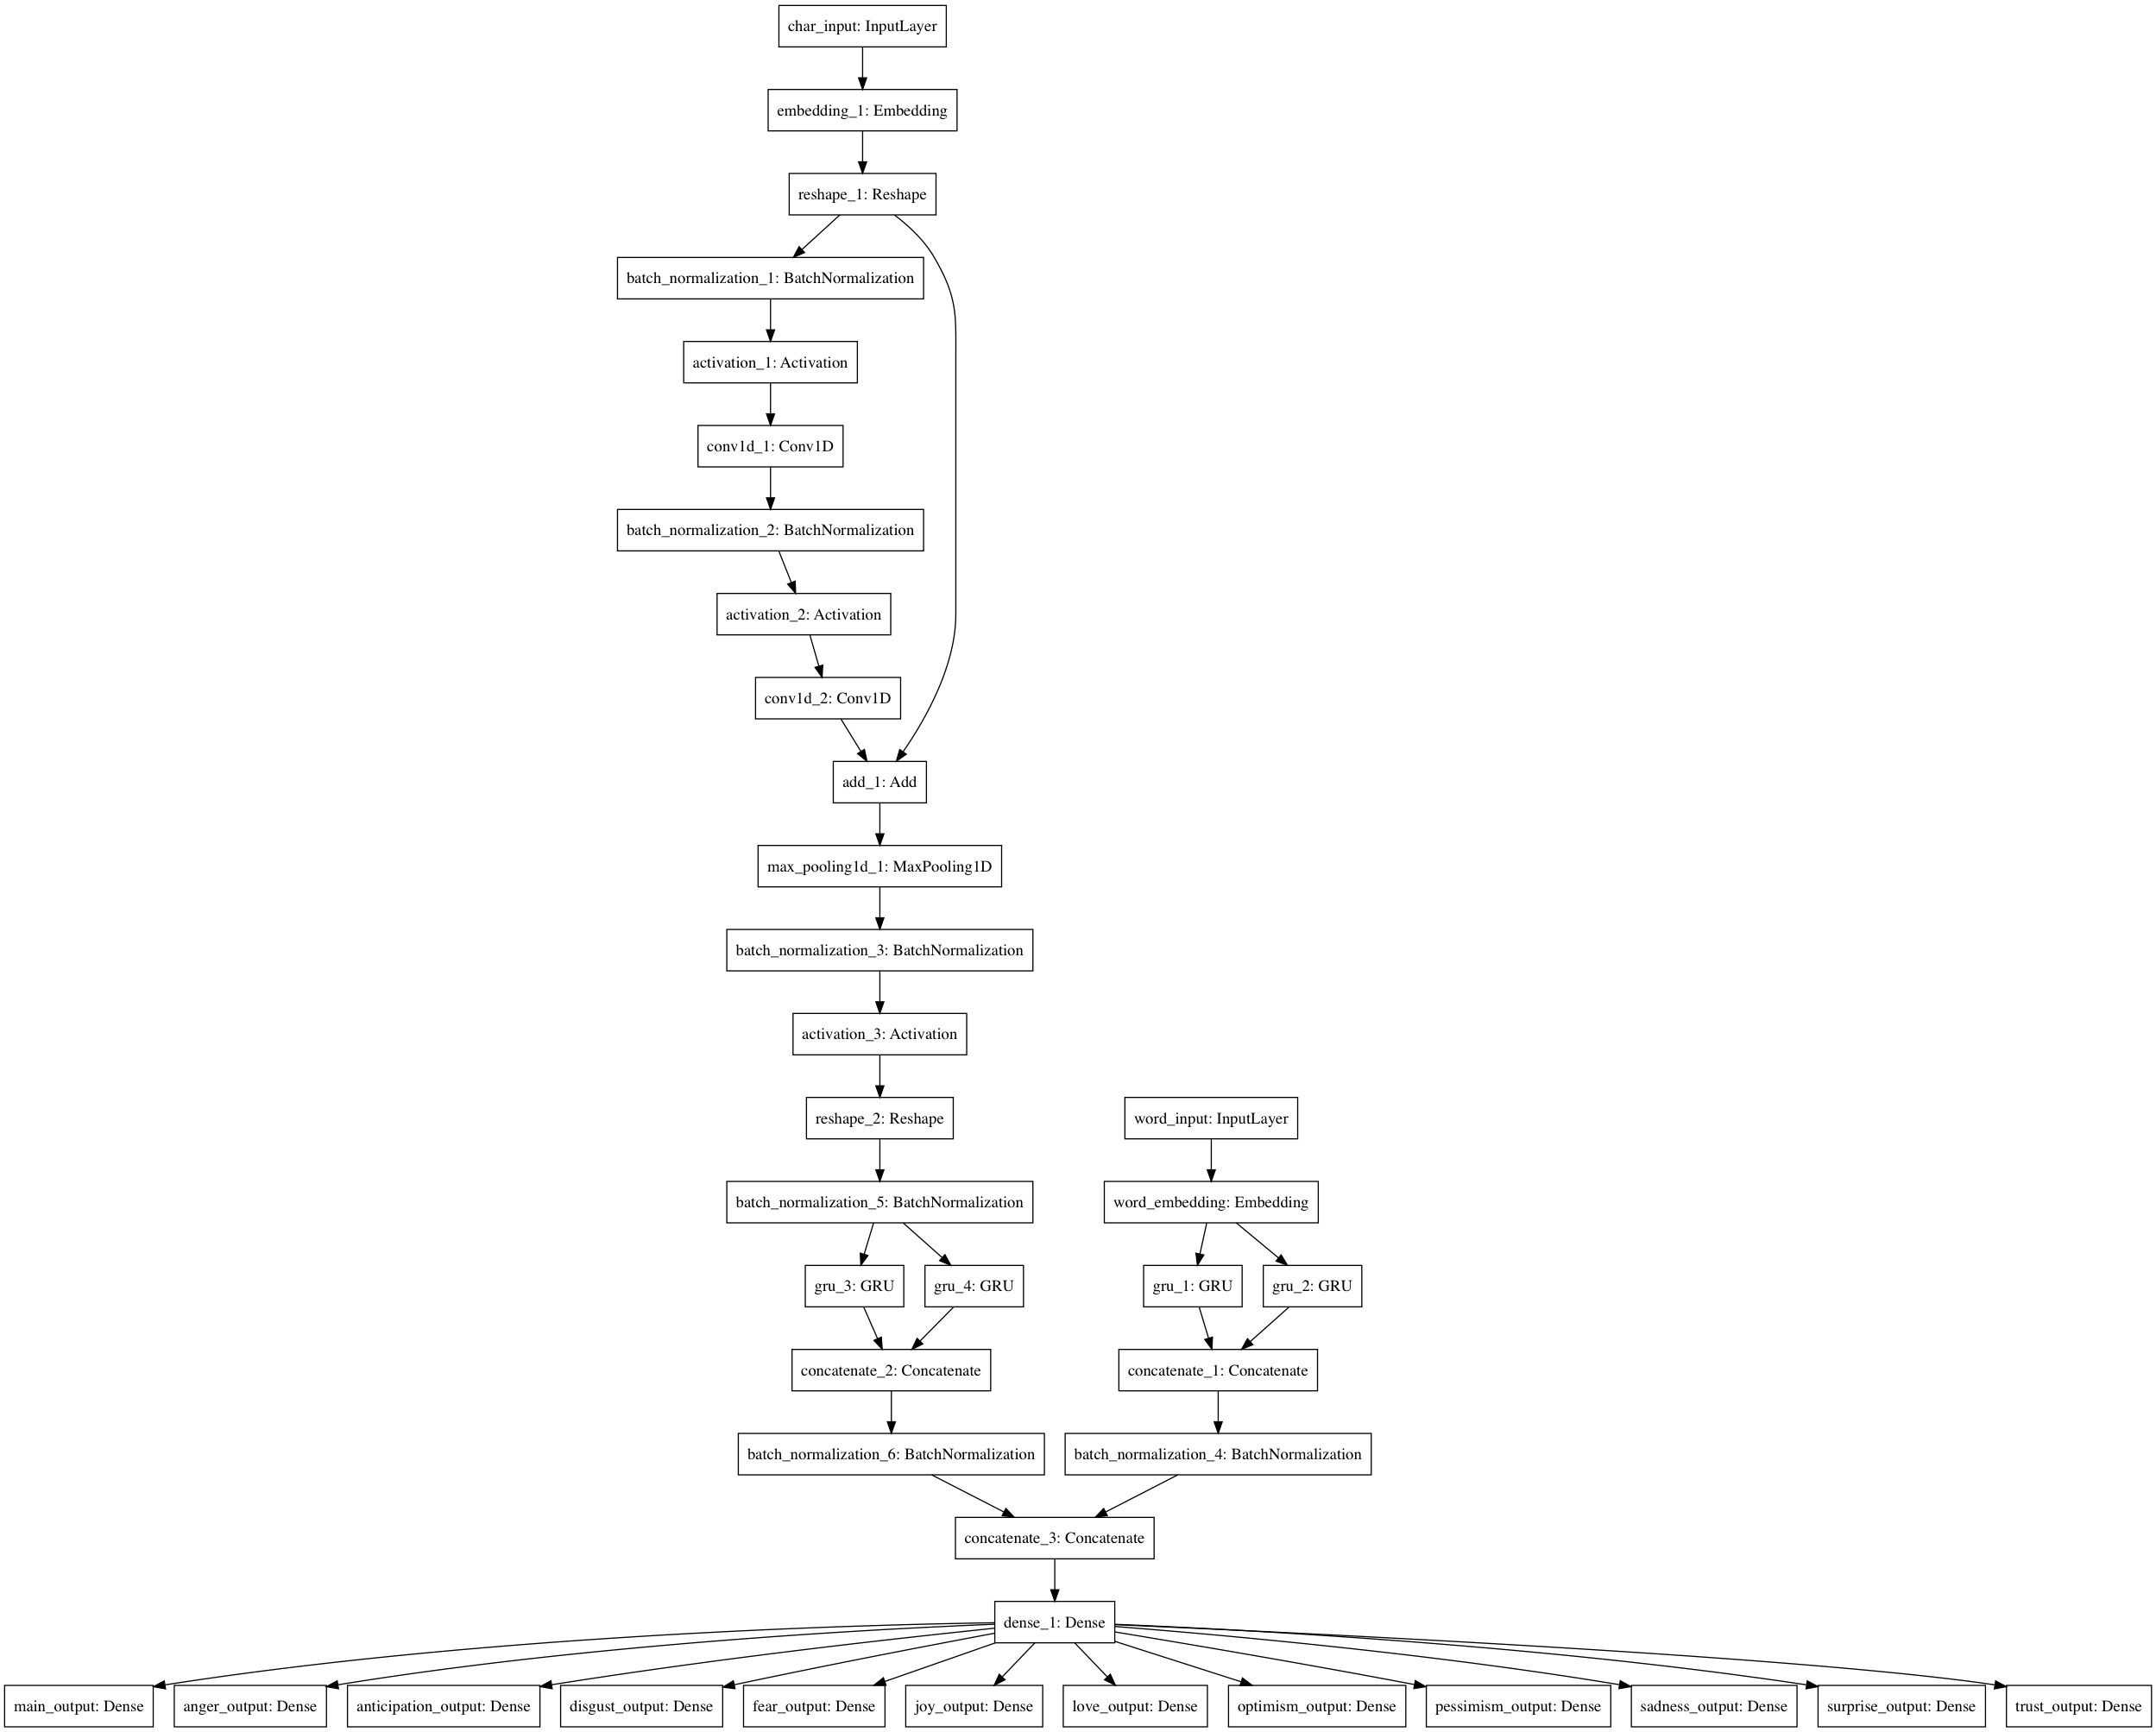
\includegraphics[width=\textwidth]{pictures/model.png}
        \caption{The full model, training on both word and character representations}
        \label{fig:fullmodel}
\end{figure}

\subsection{Model output}
Since the model reads in all regression data in one single input and outputs it in a similar bulk manner, the overall feeling from the regression data can not be intrinsically inferred from the regression value, meaning, the way that an "anger tweet" is classified as an anger tweet is its position in the large output matrix. That way, if a completely new tweet would be presented to the model, the value of the regression would be an emotion intensity felt by the tweeter but in a general sense. To help guide the intensity in a direction, the eleven classification labels could be used to infer the tweeters general state of mind. 

\subsection{Loss functions}
Since the model is a multitask model, more than one loss function was needed. The model solves two tasks which can not share loss functions, because of the inherent nature of the problem. One is a regression problem and the other a classification.

\subsubsection{Regression loss function and metric}
For the regression output of the model, mean squared error was chosen as a way to optimize the model with regards to Pearson-score. Mean squared error is used in the following form:\\
\begin{equation} \label{eq:lreg}
L_{reg}(gold, pred)=\dfrac{1}{b_{size}}\sum^{b_{size}}_{i=1}\left(gold_{i}-pred_{i}\right)^{2}
\end{equation}\\
The Pearson correlation coefficient is calculated thus in the evaluation of the scores:\\
\begin{equation} \label{eq:pearson}
r_{p} = \dfrac{\sum \left(gold-m_{gold}\right) \left(pred-m_{pred}\right)}{\sqrt{\sum \left(gold-m_{gold}\right)^{2} \left(pred-m_{pred}\right)^{2}}},
\end{equation}\\
where \textit{gold} is the truth/gold labels,\textit{pred} is the predictions and \textit{m} is the mean of the vectors subscripted.\\
There are two aspects of getting a good correlation score, i.e. a score of one. This is done by having predictions close to the gold score but also having a mean prediction similar to the gold scores. Getting a mean prediction similar to the mean gold does not necessarily coincide with having similar values. Both of these features will get reduced the closer the prediction values get to the gold values, and therefore the mean squared error proved useful in solving the specific task.\\
\\
The metric used for the regression is mean absolute error:\\
\begin{equation} \label{eq:meanabs}
m_{reg}=\dfrac{1}{b_{size}}\sum^{b_{size}}_{i=1}abs\left(gold_{i}-pred_{i}\right)
\end{equation}\\
Where $b_{size}$ is the batch size used by the model during training. 

\subsubsection{Classification loss function and metric}
The loss function for the classification is a bit more convoluted since all regression tweets have regression labels but not all regression tweets have classification labels. This is handled by way of a mask and the augmentation specified in section \ref{sec:augm}. The loss function is described as such:\\
\begin{equation} \label{eq:fclass}
f(gold,pred) =
     \begin{cases}
       0, &\quad\text{if gold = mask}\\
       wbce(gold,pred), &\quad\text{otherwise} \\
     \end{cases}
\end{equation}\\
where \textit{wbce} is our custom weighted binary cross entropy function. Since the model has eleven output layers, there is a loss function for each of the eleven emotions/layers. The function (\ref{eq:fclass}) is used in a batch wise manner as in the regression case on each emotion:\\
\begin{equation} \label{eq:lemotion}
L_{emotion}=\dfrac{1}{b_{size}} \sum_{i=1}^{b_{size}} f(gold_i, pred_i)
\end{equation}\\
 This loss function ensures that tweets with no classification labels do not impact the updating of the weights of the model by giving the predicted values a loss of zero.\\
Binary cross entropy is defined as follows:\\
\begin{equation}
BCE(gold,pred) = -(gold \cdot log(pred)+(1-gold) \cdot log(1-pred))
\end{equation}\\
The custom weighted binary cross entropy function is defined as follows:\\
\begin{equation} \label{eq:wBCE}
wBCE(gold,pred) = (gold \cdot 1_{weight} + (1-gold) \cdot 0_{weight}) \cdot BCE(gold, pred)
\end{equation}\\
where $1_{weight}$ and $0_{weight}$ are parameters that can be tuned in the model. This weighting parameter is included because of the uneven distribution of ones and zeros. The goal of the model is to detect whenever emotions are felt by the tweeter, and as such ones are to be valued more if guessed.  \\ \\
The metric used for classification is a custom metric function which builds on binary accuracy. The custom part consists of masking the -1's the same way as the loss function, so that the metric returns a value corresponding to a correct guess whenever classification labels are missing. The custom metric function looks like this: \\
\begin{equation}
f(gold,pred) =
     \begin{cases}
       1, &\quad\text{if gold = mask}\\
       BA(gold,pred), &\quad\text{otherwise} \\
     \end{cases}
\end{equation}\\
where \textit{BA} is defined as follows: \\
\begin{equation} \label{eq:bin_acc}
BA(gold, pred) =
	\begin{cases}
		1, &\quad\text{if gold = round(pred)} \\
		0 &\quad\text{otherwise} \\
	\end{cases}
\end{equation}\\
where the \textit{pred} value is rounded to 0 or 1 since it is a probability value of the guessed emotion.\\
This equation is then used and averaged batch-wise like the loss: \\
\begin{equation} \label{eq:class_metric}
m_{class}=\dfrac{1}{b_{size}}\sum^{b_{size}}_{i=1}f\left(gold_{i}-pred_{i}\right)
\end{equation}\\

\subsubsection{Combined loss function}
The model is trained using the sum of equation (\ref{eq:lreg}) and (\ref{eq:lemotion}):\\
\begin{equation} \label{eq:lratio}
L_{combined}(gold,pred)=L_{ratio}\cdot L_{reg}(gold, pred) +  \sum_{e\in E}\dfrac{(1-L_{ratio})}{|E|}\cdot L_{e}(gold, pred),
\end{equation}\\
where \textit{e} is one of the eleven emotions in \textit{E}. The ratio $L_{ratio}$ is a parameter that can be tweaked and can be used to force the model implicitly to weight one task higher than the other. Furthermore, the weighting of the single classification emotions can also be tweaked and given more weighting than the others.

\subsection{Hyperparameter testing}
\subsubsection{Regression, task 1}
In figure \ref{fig:averagedropout} the Pearson score is plotted with regards to the different dropout values.
\begin{figure}[H]
    \centering
        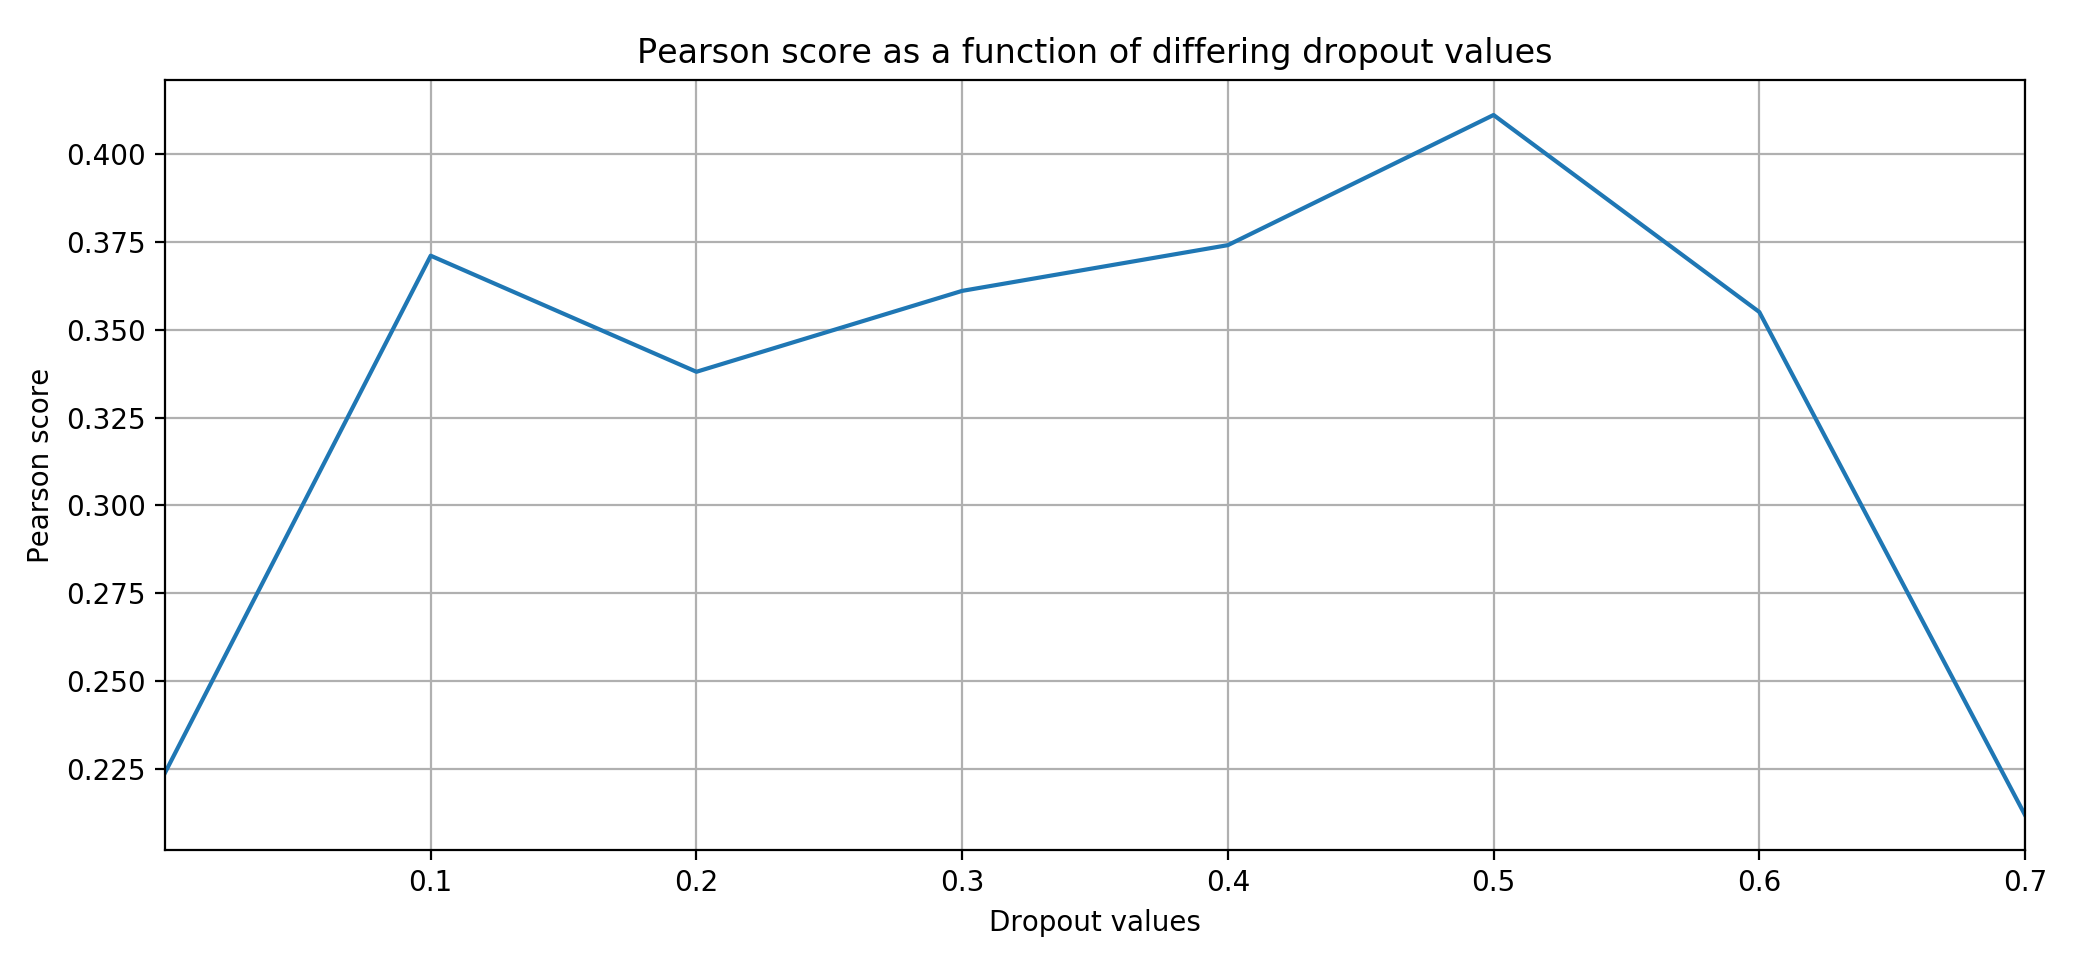
\includegraphics[width=\textwidth]{pictures/DropoutPlot.png}
        \caption{Pearson scores as a function of dropout value, loss weight set to 0.45, weighted BCE set to 0.5}
        \label{fig:averagedropout}
\end{figure}
It is evident that dropout values higher than 0.5 results in worse Pearson scores. This is because of the models tendency to underfit because of the sheer amount of hidden units getting dropped in every run. Furthermore, predictions on joy is significantly worse than the other regression emotions.\\
\\
The weighting in the binary cross entropy, as used in equation (\ref{eq:wBCE}) still has an interplay with the Pearson score reached by the model, since the two tasks are solved jointly, as thus this correlation is relevant.
\begin{figure}[H]
    \centering
        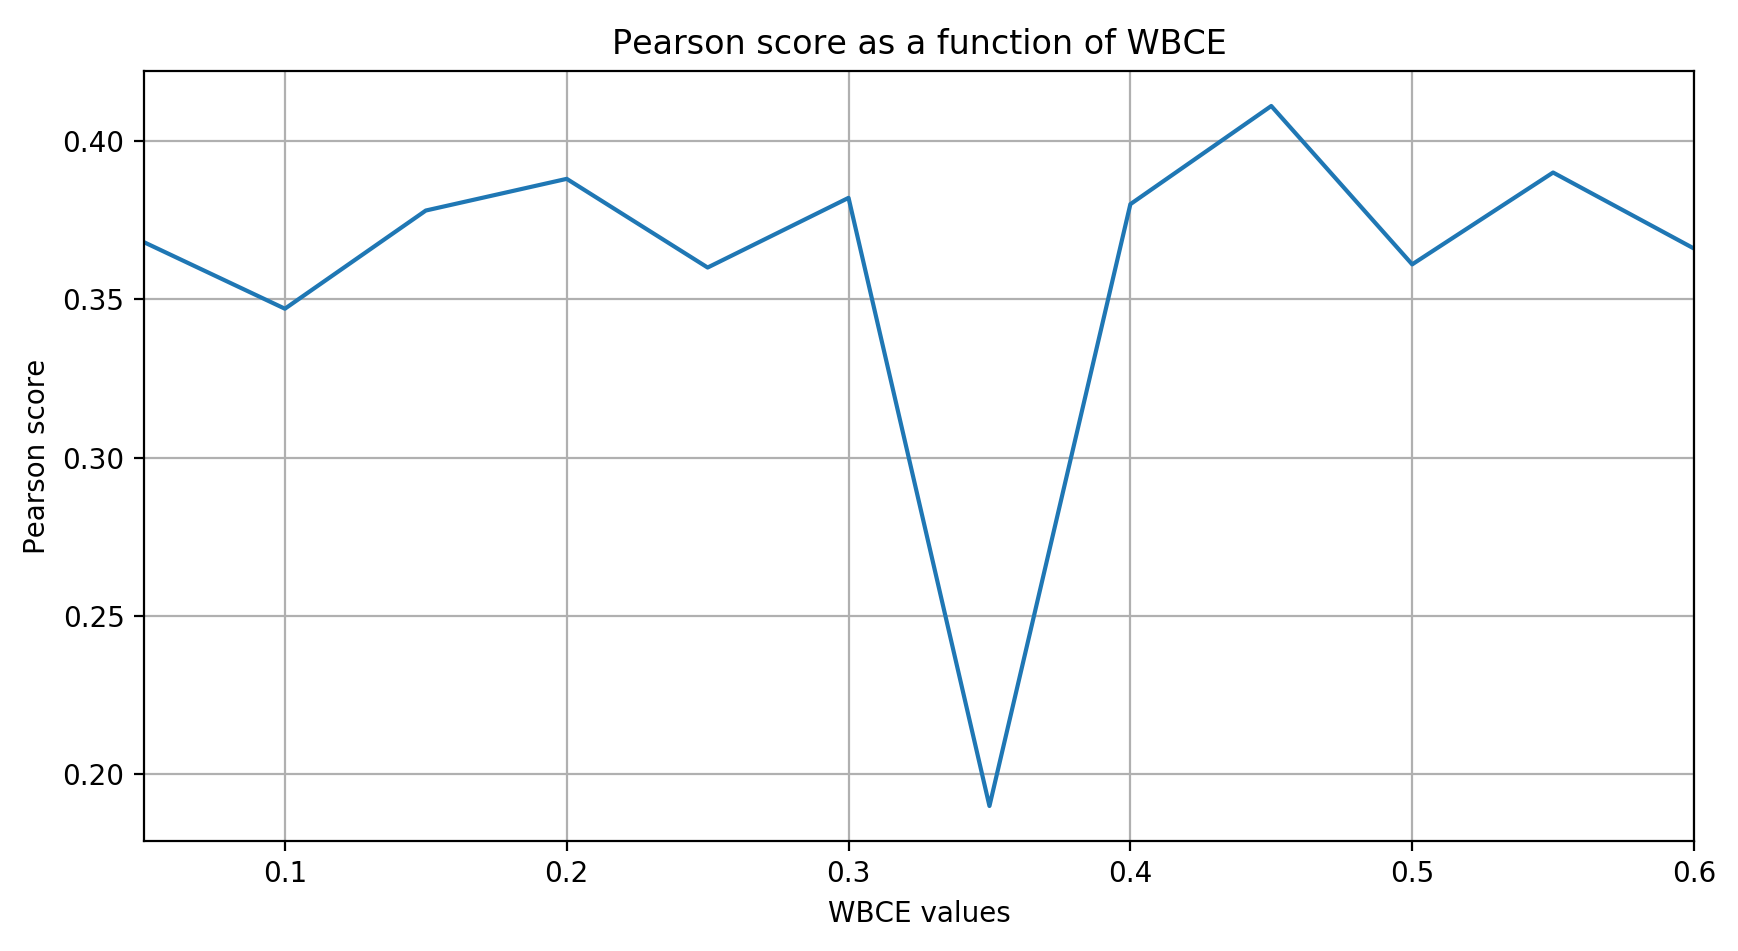
\includegraphics[width=\textwidth]{pictures/weightedBCEplot.png}
        \caption{Average Pearson score as a function of weighted BCE value, dropout set to 0.3, loss weight set to 0.45}
        \label{fig:averageBCE}
\end{figure}
The weightings shown in figure \ref{fig:averageBCE} is the weight of the zeros and the one weights are then $1-0_{weight}$, as outlined in equation (\ref{eq:wBCE}).\\
In figure \ref{fig:averageBCE} it can be seen that the effect of the weighting is not wholly insignificant. The best Pearson score is reached with a weighting of zeros to 0.45 and ones to 0.55. Beyond a weight of 0.6, that is, weighting zeros 0.6 and ones 0.4 the Pearson score started dropping off. It is unclear why the outlier at a weighting of 0.35 deviates so much from the general tendency, since the model and predictions were healthy, albeit very bad.\\
\\
The loss weights plotted in figure \ref{fig:averageLW} are the loss weights as outlined in equation (\ref{eq:lratio}).
\begin{figure}[H]
    \centering
        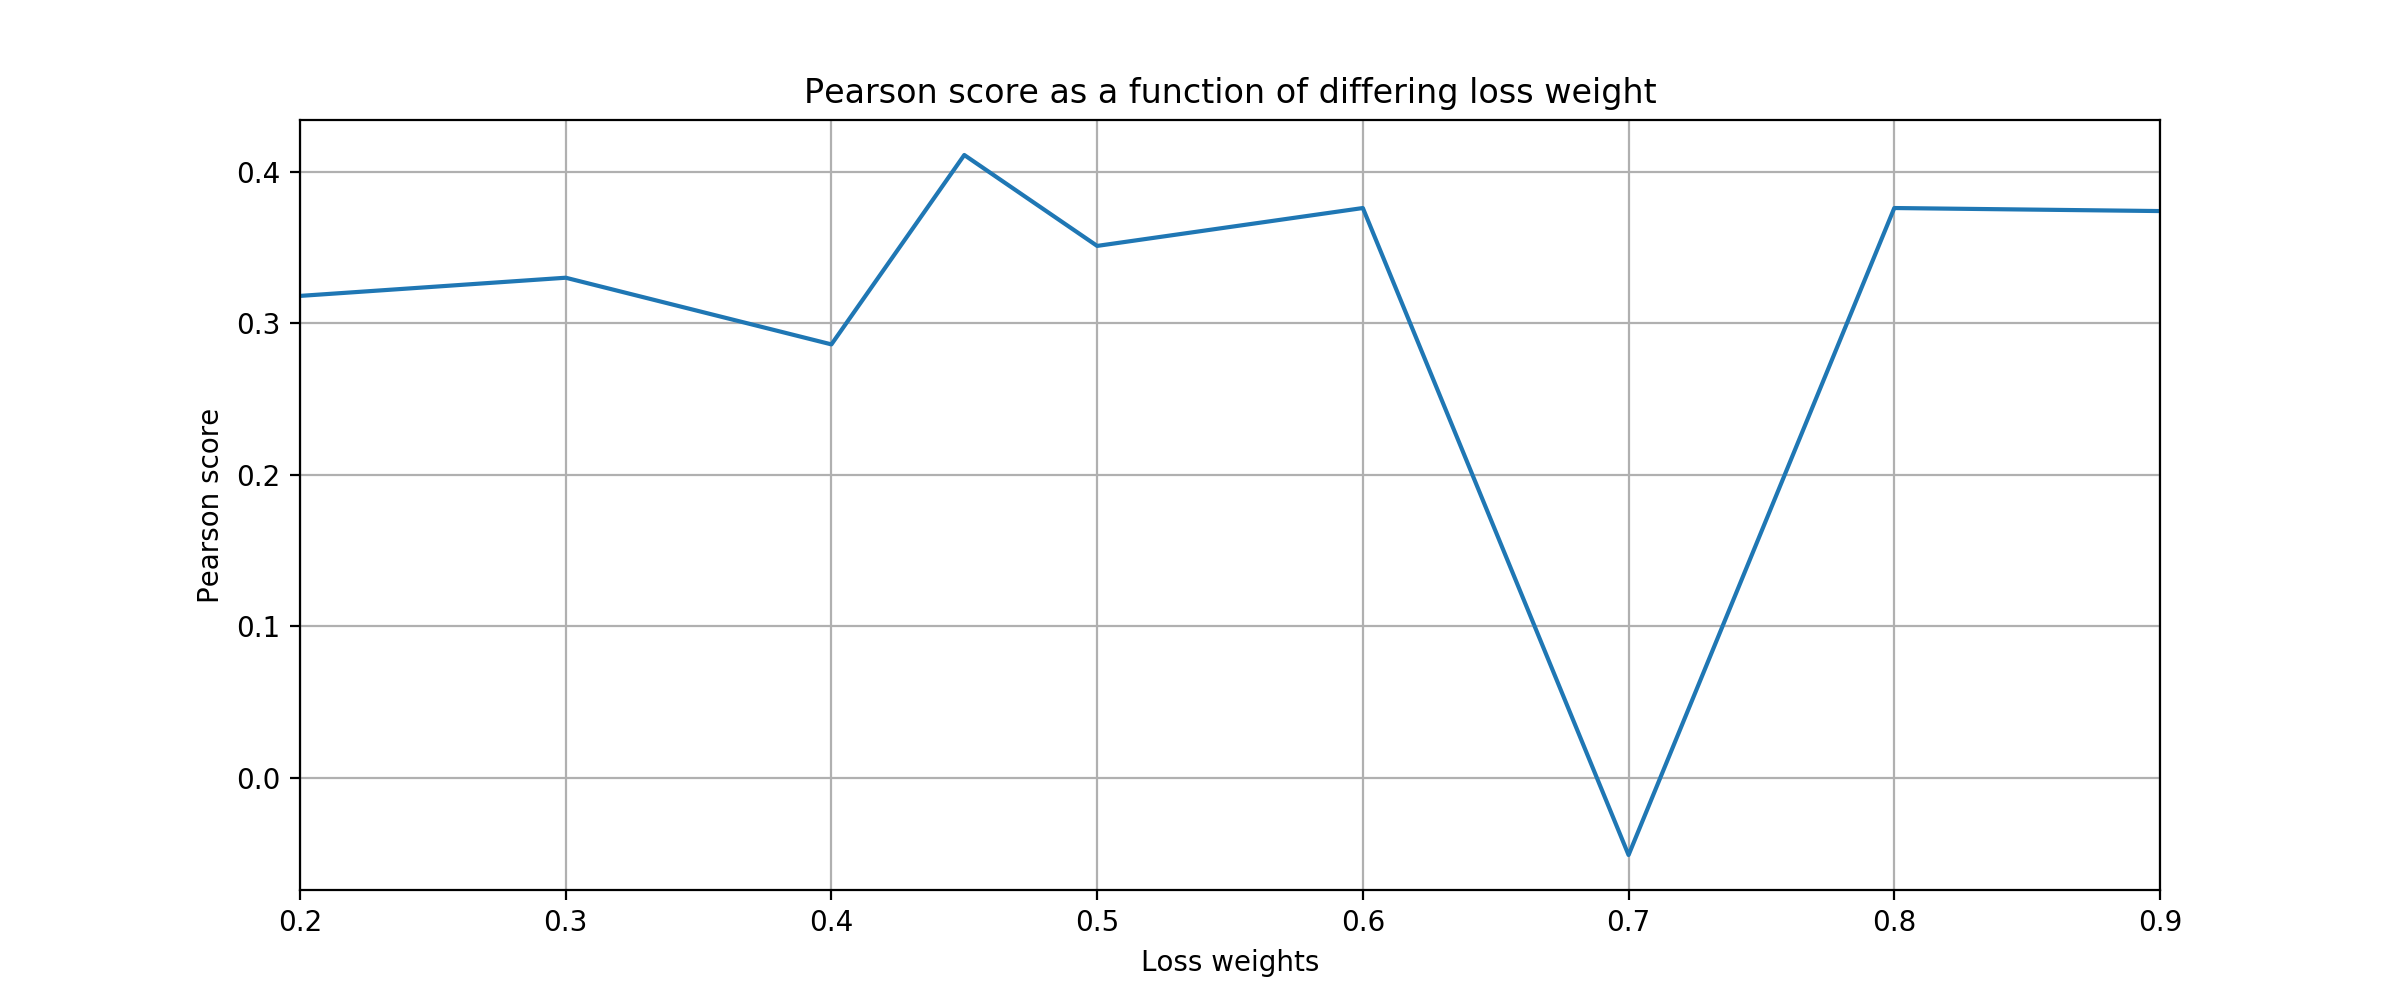
\includegraphics[width=\textwidth]{pictures/LossWeightsPlot.png}
        \caption{Average Pearson scores as a function of loss weight value, dropout set to 0.3, weighted BCE set to 0.45}
        \label{fig:averageLW}
\end{figure}
The loss weights have an outlier, and much like the outlier in the testing of weights for the binary cross entropy, is it unclear why it is present as the model guessed in the correct form, just badly.\\
The general tendency of the loss weights was not fully as to be expected, meaning, a high weighting towards the regression task would yield a better Pearson score. This might have to do with the fact that the embedding weights being trained to do minimize the weighted sum of the two loss function (equation (\ref{eq:lratio})) might not favor one task heavily over the other, i.e. the two tasks have an overlap in the weights that solve them and in the overall structure of the tasks.

\begin{table}[h]
\centering
\begin{tabular}{c|c|c|c|c|c|}
& \text{Anger} & \text{Fear} & \text{Joy} & \text{Sadness} & \text{Avg.} \\ \hline
\text{No embedding} & 0.249 & 0.471 & 0.208 & 0.362 & 0.323 \\
\text{Embedding} & 0.382 & 0.520 & 0.108 & 0.434 & 0.361
\end{tabular}
\caption{Pearson scores with and without pre-trained word embeddings}
\label{tab:no_emb}
\end{table}

From table \ref{tab:no_emb}, it is clear that embeddings give  a better score than no embeddings, although one noticeable difference is the Pearson score for joy. This could have something to do with the pretrained embedding weights not having a good instantiation towards the more positively weighted words, which then skews the results for that particular emotion.  

\begin{table}[h]
\centering
\begin{tabular}{c|c|c|c|c|c|}
& \text{Anger} & \text{Fear} & \text{Joy} & \text{Sadness} & \text{Avg.} \\ \hline
\text{NADAM} & 0.282 & 0.480 & 0.205 & 0.373 & 0.335 \\
\text{ADAM} & 0.405 & 0.457 & 0.150 & 0.429 & 0.360
\end{tabular}
\caption{Pearson scores with NADAM and ADAM optimizers}\label{tab:NADAM_ADAM}
\end{table}

Some light testing was done in way of optimizers used for the model. The final choice of optimizer was the ADAM optimizer with a learning rate of 0.001, a learning rate decay of $10^{-5}$ and clipping the gradients to 1. The only difference between the two optimizers was that NADAM used Nesterov momentum. Explaining the difference and going in-depth with optimizers is beyond the scope of this report, and only superficial tests were done between the two. \\
\\
More detailed barplots of the different runs can be seen in the appendix, figures \ref{fig:dropoutvalues}, \ref{fig:BCEvalues} and \ref{fig:LWvalues}.
\subsubsection{Classification, task 5}
In figure \ref{fig:dropoutacc} the accuracy is plotted with regards to the dropout values.
\begin{figure}[H]
    \centering
        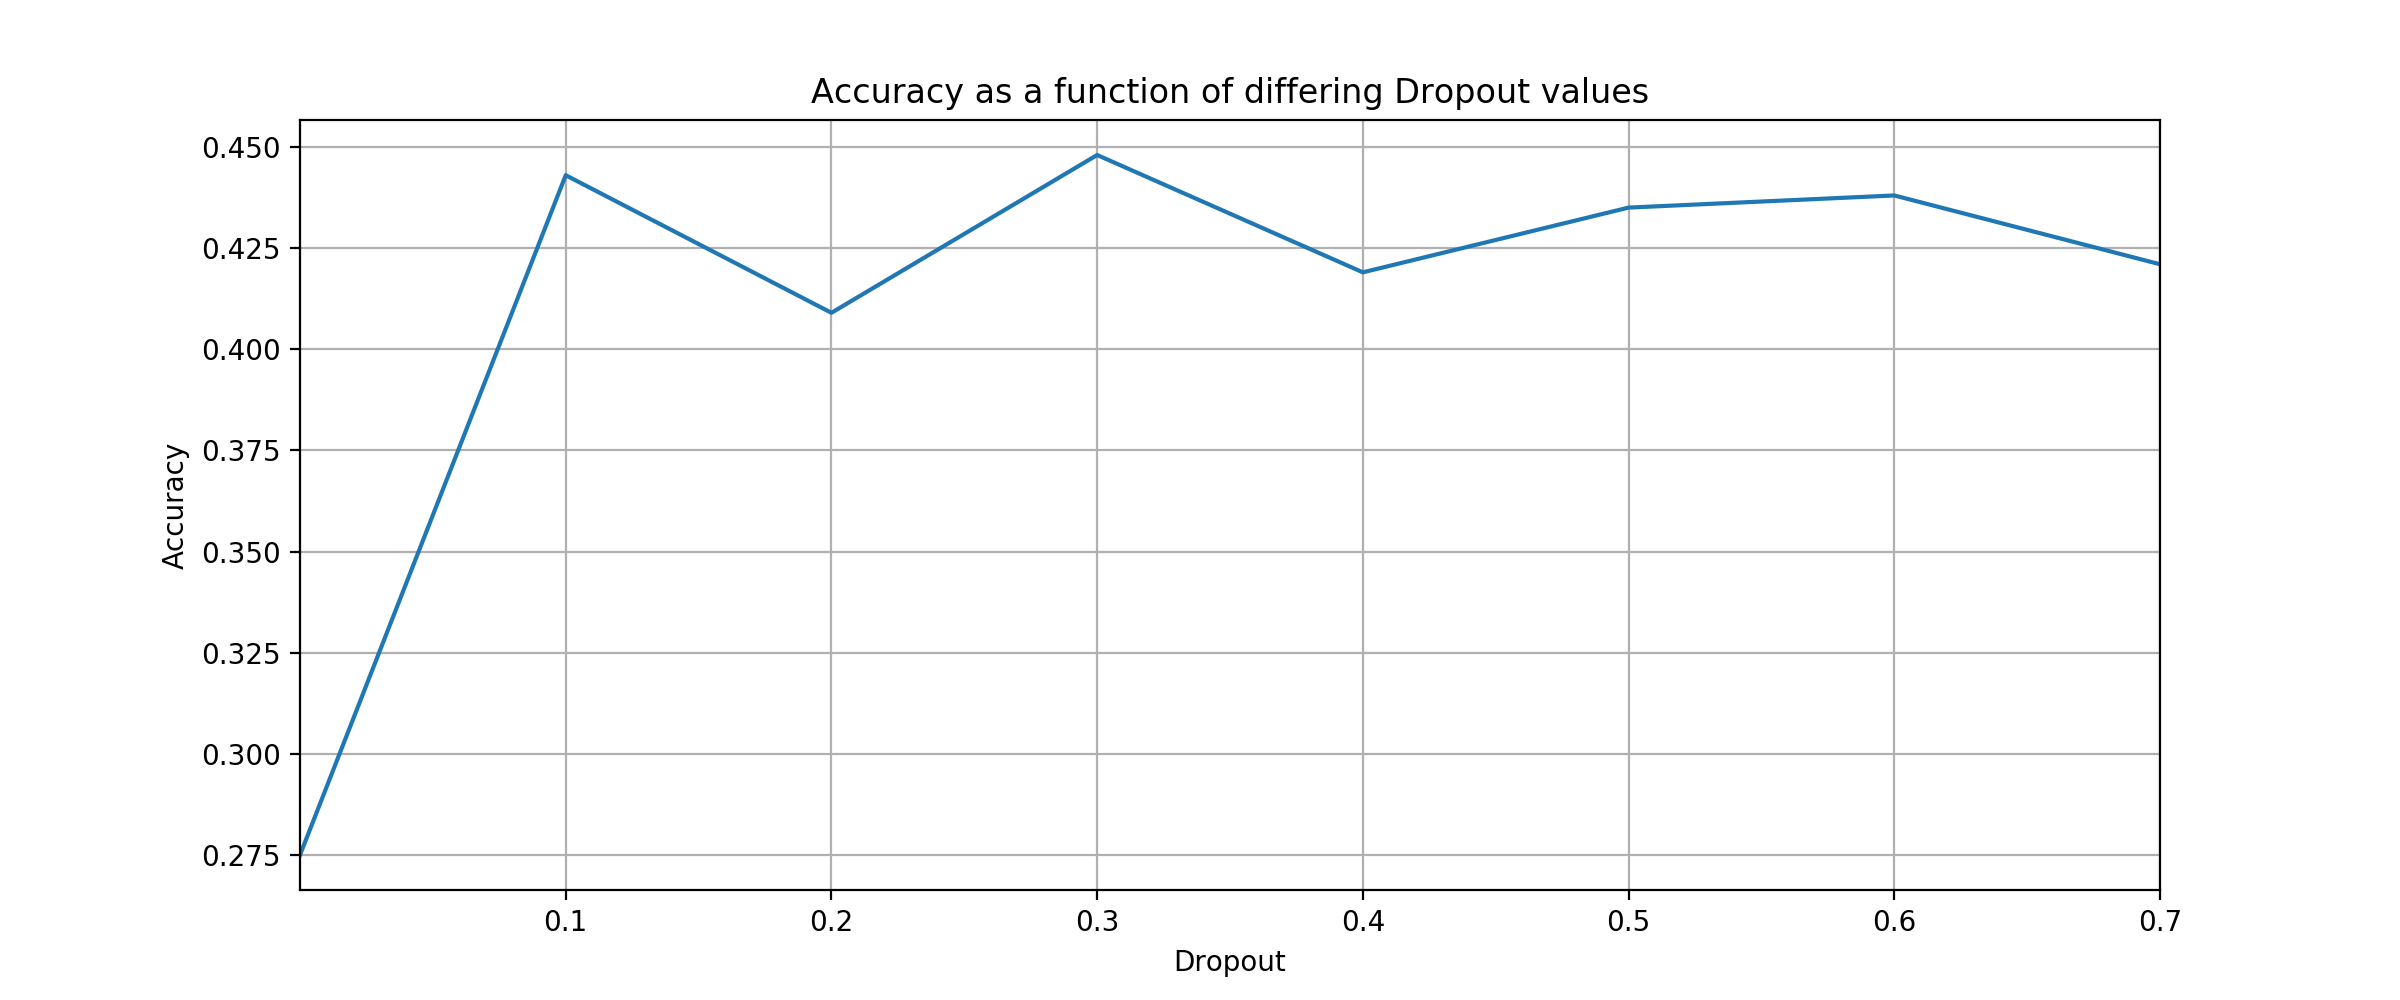
\includegraphics[width=\textwidth]{pictures/DropoutPlotAcc.png}
        \caption{Accuracy as a function of dropout value, loss weight set to 0.45, weighted BCE to 0.45}
        \label{fig:dropoutacc}
\end{figure}
As seen in the regression case, some dropout is needed, but there is not a clear tendency whether or not a specific dropout value is significantly better than the others.\\
\\
In figure \ref{fig:bceacc} the accuracy is plotted with regards to the different weighted BCE values.
\begin{figure}[H]
    \centering
        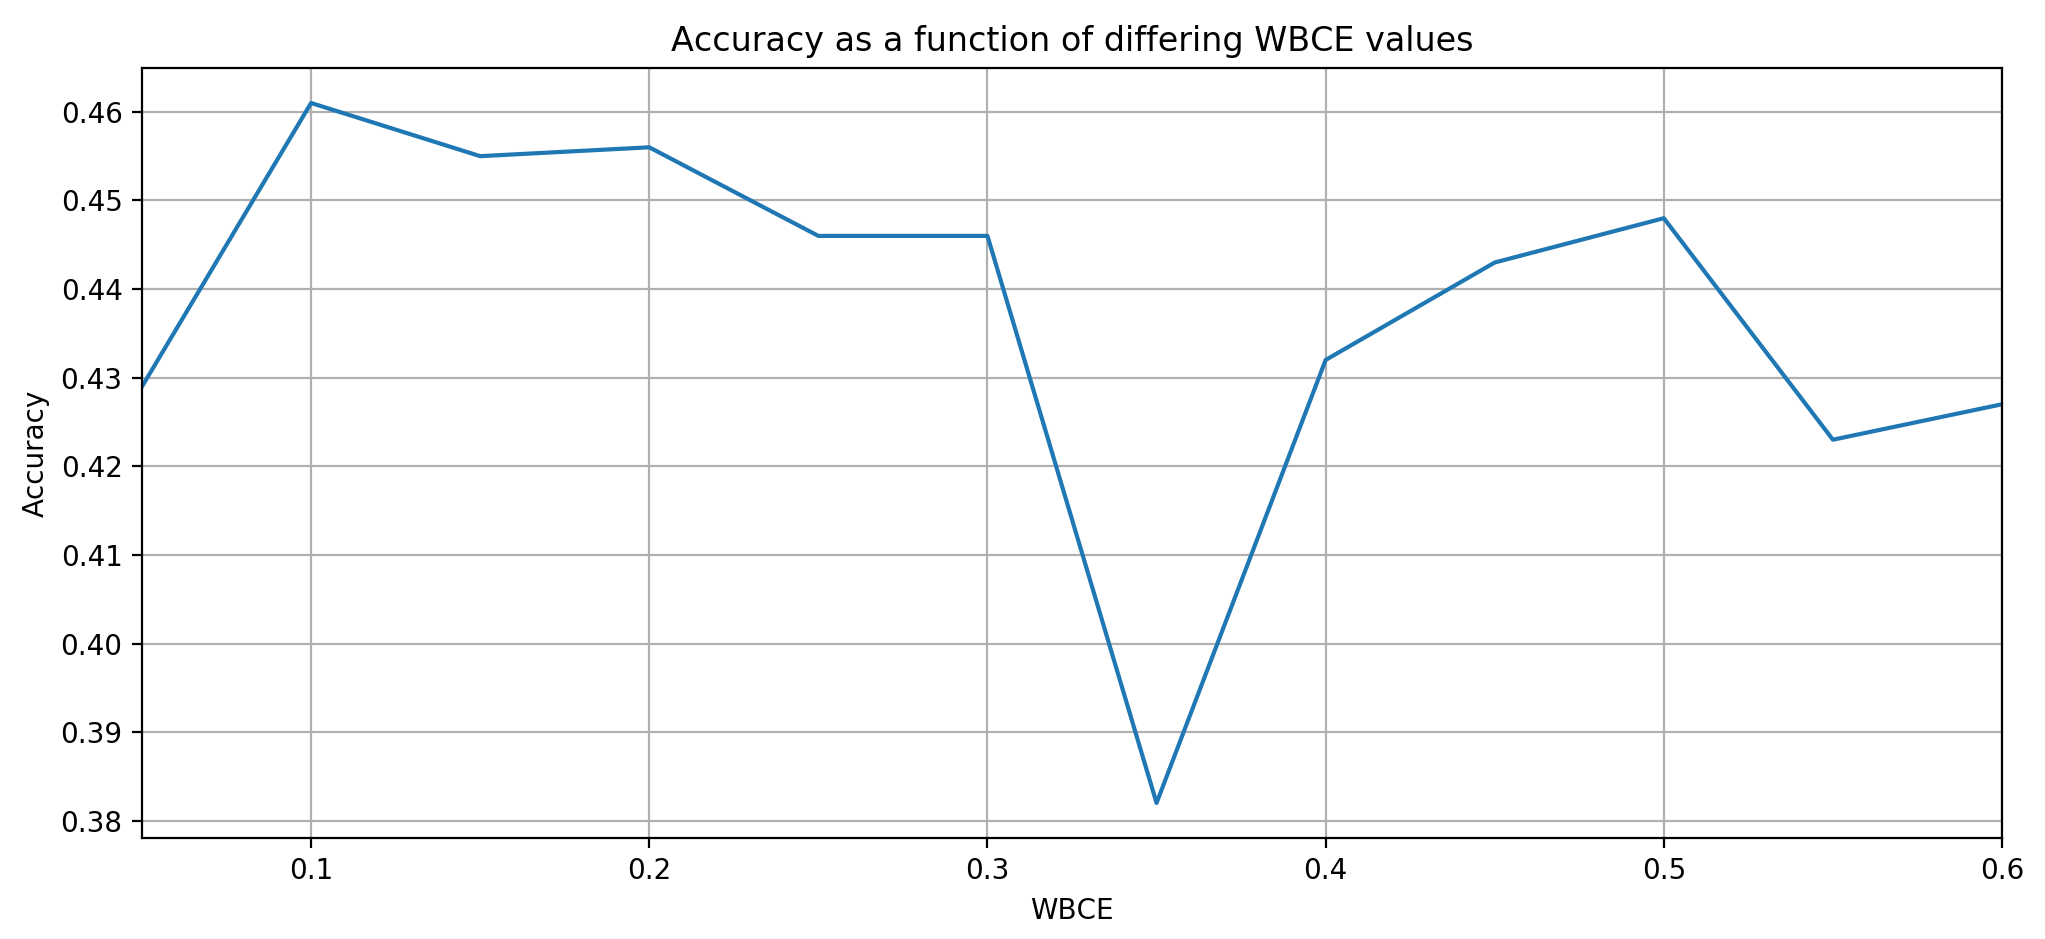
\includegraphics[width=\textwidth]{pictures/WBCEPlotAcc.png}
        \caption{Accuracy as a function of weighted BCE value, loss weight set to 0.45, dropout set to 0.3}
        \label{fig:bceacc}
\end{figure}
As can be seen in figure \ref{fig:bceacc}, there is an outlier at a weighted BCE value of 0.35. It is also noticeable that at a weighted BCE value of 0.1, meaning that a weighting of zeros to a tenth of the summed loss contribution, the accuracy gets noticeably better. This value was not chosen, however, as it drastically reduced the Pearson score of the model, as seen in figure \ref{fig:averageBCE}, the overall loss would then be worse. \\
\\
In figure \ref{fig:lwacc} the accuracy is plotted with regards to the different loss weight values. 
\begin{figure}[H]
    \centering
        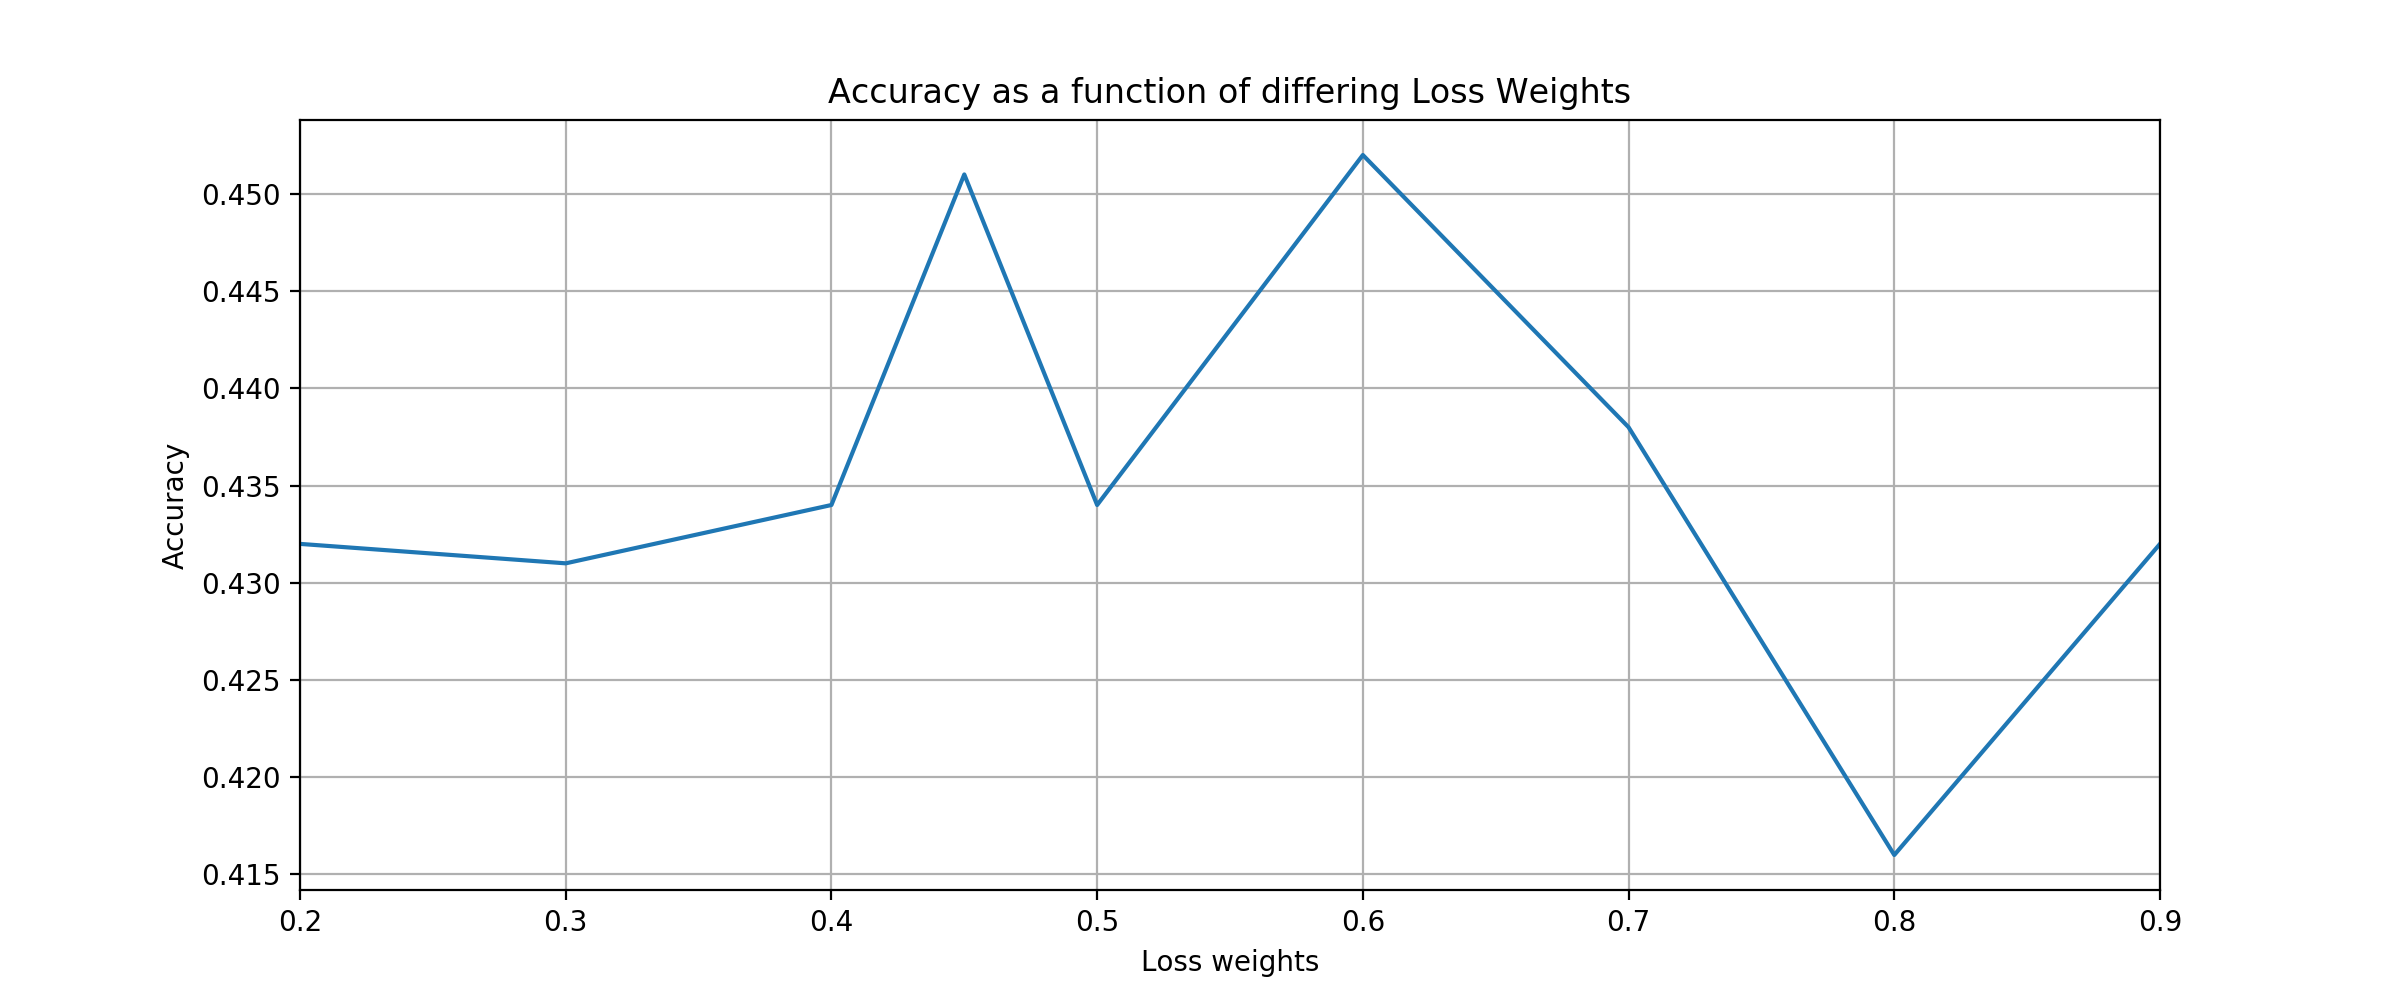
\includegraphics[width=\textwidth]{pictures/LossWeightPlotAcc.png}
        \caption{Accuracy as a function of loss weight value, weighted BCE set to 0.45, dropout set to 0.3}
        \label{fig:lwacc}
\end{figure}
As with the regression case, the Pearson score at the different loss weights would be expected to have a larger impact.

\subsection{Results and data}
The final model used was zeroed in on through an experimental basis. It used $0_{weight}=0.45$ and $1_{weight}=0.55$, a dropout of 0.5 and $L_{reg}=0.45$ and $L_{class}=0.55$. 400 dimensional word and char embeddings and a 250 dimensional GRU was used for each submodel. The resulting sanity check yielded following results:
\begin{table}[H]
\centering
\begin{tabular}{c|c|c|c|c}
\text{Anger} & \text{Fear} & \text{Joy} & \text{Sadness} & \text{Avg.} \\ \hline
0.865 & 0.896 & 0.882 & 0.897 & 0.885 \\
\end{tabular}
\caption{Sanity check Pearson scores for regression}
\label{tab:sanityreg}
\end{table}

\begin{table}[H]
\centering
\scalebox{0.7}{\begin{tabular}{c|c|c|c|c|c|c|c|c|c|c|c|c}
\multicolumn{12}{c}{\textbf{F-micro}} & \textbf{Global accuracy}\\ \hline
Anger & Anticipation & Disgust & Fear & Joy & Love & Optimism & Pessimism & Sadness & Surprise & Trust & Neutral & \\ \cline{1-12}
0.968 & 0.931 & 0.964 & 0.971 & 0.982 & 0.931 & 0.955 & 0.899 & 0.951 & 0.909 & 0.905 & 0.833 & 0.933 \\
\end{tabular}}
\caption{Sanity check scores for classification}
\label{tab:sanityclass}
\end{table}
The results of the final model on the development data is shown in tables \ref{tab:devreg} and \ref{tab:devclass}.

\begin{table}[H]
\centering
\begin{tabular}{c|c|c|c|c}
\text{Anger} & \text{Fear} & \text{Joy} & \text{Sadness} & \text{Avg.} \\ \hline
0.371 & 0.555 & 0.184 & 0.532 & 0.411 \\
\end{tabular}
\caption{Pearson scores for regression on development data}
\label{tab:devreg}
\end{table}

\begin{table}[H]
\centering
\scalebox{0.7}{\begin{tabular}{c|c|c|c|c|c|c|c|c|c|c|c|c}
\multicolumn{12}{c}{\textbf{F-micro}} & \textbf{Global accuracy}\\ \hline
Anger & Anticipation & Disgust & Fear & Joy & Love & Optimism & Pessimism & Sadness & Surprise & Trust & Neutral & \\ \cline{1-12}
0.687 & 0.232 & 0.626 & 0.638 & 0.685 & 0.416 & 0.574 & 0.179 & 0.555 & 0.141 & 0.038 & 0.053 & 0.443 \\
\end{tabular}}
\caption{Classification scores on development data}
\label{tab:devclass}
\end{table}


% !TeX root = ../report.tex

\section{Discussion}

\subsection{SemEval Task}
\subsubsection{Reusing tweets}
The full amount of unique tweets between task 1 and 5 is not easily inferable, but some rules can be deduced:\\
\begin{itemize}
\item All classification tweets are unique
\item All classification tweets have a regression label, but not vice versa
\item A tweet can appear in multiple regression emotions
\end{itemize}
Since the model is trained on the full 7102 regression tweets, two tweets with differing regressional values and feelings could map to the same classification labels. This can leave the model predicting ambiguously, since the same classification labels get associated with differing regression labels, words and character representations. This effect was not countered in any meaningful way, since it was not considered to be too disruptive. The effect could be countered by only selecting unique tweets, but this would then start interfering with the data given for the subtasks, and start losing relevance with regards to the tasks. 

\subsection{Feature based}
\subsubsection{Custom features and effect}
For the feature based approach, six custom features were used:
\begin{itemize}
\item Exclamation: check whether or not an exclamation mark was present in the tweet.
\item Hashtag: check whether or not an hashtag was present in the tweet.
\item Spelling: check whether or not are specified percentage of the tweet was mispelled.
\item Negative emoji: check whether or not an emoji from a list of negative emojis was present in the tweet.
\item Positive emoji: check whether or not an emoji from a list of positive emojis was present in the tweet.
\item Emoji: check whether or not an emoji was present in the tweet.
\end{itemize}
All these custom features are boolean in nature; they consist of a check for whether or not a condition holds. This is a result of the relative ease with which one can engineer such features. The only value that would need any tweaking would be the ratio with which the spelling feature would be set, and this was deduced on a purely experimental basis. To a certain degree the positive and negative emojis are also a question of selecting and agreeing on which emojis are inherently positive and negative, but these were kept short and rather general.

\subsection{Deep learning}
\subsubsection{What should the model do and how should it do it?}
A choice was taken early in the process that the model should be as general as possible and take as much data with differing truth labels as possible. The model, as of now, takes the truth labels from task 1 and task 5. These two tasks were chosen because of their relatedness with regards to emotion inference from tweets, but difference in that they require regression and classification. The difference between task 1 and task 2 seem trivial, in that a mapping from a 0-to-1 regressional value can be mapped to an ordinal classification with relative ease, but the mapping from 0-to-1 regressional value to 11 binary flags, indicating emotions felt or not, seemed to require a more elaborate structure and loss function balancing.\\
\\
One thing of note is the way the data from task 1 is used in the final model. The regressional values are indirectly interpreted more as the outputs of a model trying to solve task 3 (\textit{Given a tweet, determine the intensity of sentiment or valence (V) that best represents the mental state of the tweeter—a real-valued score between 0 (most negative) and 1 (most positive)}) since emotionality is stripped implicitly. This is not the objective this data has been annotated towards, this has been annotated with regards to 4 specific emotions, but since the emotion of these scores are not directly evident from the output of the model, the scores can be considered to be more directly dependent of the classification label outputs. This is not the necessarily the most meaningful way of guessing emotion intensities but it makes sense within the context of the task the model solves.

VI SKAL SKRIVE MERE.\\

\subsubsection{Model iterations} \label{sec:iter}
The first baby steps towards a multi task learning model was reached by solving the regression task first and having a secondary output which consisted of a 4 dimensional vector with sigmoid activation and a single output using a softmax layer which indicated which regression emotion was felt. This classification was easily implemented since the truth labels were readily available because of the regression task needing 4 different emotion groupings. This way of classifying tweets could be reintroduced as to avoid the ambiguity of the regression value output in the models current state.\\
The first iteration of the model that attempted to solve task 5 had a different output layer/loss function constellation with regards to the classification of the tweets. It had a single, 11 dimensional output vector which corresponded to the full classification label list. This model would have a high degree of skew and very little variance, and this was the product of having a single layer with a limited amount of weights to be tweaked on. Since an average label list had a high amount of zeros (as shown in table \ref{tab:skew}) the weighting for the classification output layer would have a tendency to guess zeros and since there was not enough parameters to be tweaked the results would end up looking the same for all tweets.\\
The last, and current model iteration has 11, one-dimensional output vector, one for each classification label. The ability to tweak weights one a per-label basis ended up in the most meaningful predictions from the overall model architecture.

\subsubsection{Loss functions; how to model the classification}
As can be seen in table \ref{tab:skew}, flags are skewed towards certain emotions. This uneven distribution might have something to do with the ease of labelling a tweet with the emotions. Since the train, dev and test data for the task has been manually labelled, certain "human" effects might be felt and can be backpropagated through to the models built on the data. For instance, it might be very easy to infer anger in a tweet; an exclamation mark, a curse word or something similar might be used to infer the feeling, but how can you infer surprise? Or trust? Furthermore, 274 of the tweets had no feeling flags set, which was to be understood as a "neutral" feeling.\\
\begin{table}[h]
\scalebox{0.8}{\begin{tabular}{c|c|c|c|c|c|c|c|c|c|c|c|}
& \text{Anger} & \text{Anticipation} & \text{Disgust} & \text{Fear} & \text{Joy} & \text{Love} & \text{Optimism} & \text{Pessimism} & \text{Sadness} & \text{Surprise} & \text{Trust} \\ \hline
\text{\# of flags set} & 2605 & 990 & 2666 & 1269 & 2499 & 699 & 2007 & 812 & 2076 & 365 & 352 \\
\text{\% of tweets} & 38\% & 14\% & 39\% & 19\% & 37\% & 10\% & 29\% & 12\% & 30\% & 5\% & 5\%
\end{tabular}}
\caption{The actual flags set and percentage of the full classification dataset}
\label{tab:skew}
\end{table}\\
\\
The following is the main metric used for classification in the official SemEval task:\\
\begin{equation} \label{eq:accuracy}
Accuracy = \dfrac{1}{\lvert T \rvert} \sum_{t\in T}\dfrac{\lvert G_{t} \cap P_{t}\rvert}{\lvert G_{t} \cup P_{t}\rvert}
\end{equation}\\
LAV MÅSKE EN FODNOTE TIL EQUATION???\\
where $G_{t}$ is the set of the gold labels for tweet t, $P_{t}$ is the set of the predicted labels for tweet t, and T is the set of tweets. This metric can be problematic since it completely disregards tweets with zero flags set, which otherwise could present a nice and diverse understanding of feelings and their interplay on how people will write their tweets. The secondary official metrics are also problematic in that they also disregard "neutral" tweets. The secondary metrics are a combination of micro and macro precision, recall and f-scores. To mitigate this, the evaluation script used for local evaluation included a twelfth dimension which was only set if all the others were not set. This allowed for a more nuanced picture in the edge case were all of the flags were not set.

% !TeX root = ../report.tex

\section{Conclusion}
In this report, two different models were presented that both solve subtasks in SemEval-2018 Task 1. Firstly, a feature based model was presented. This model acted as an opener for the task and possible solutions to it. It presented a decent baseline for the scores and the general solving of the task. The results were subpar with regards to last years comparable results. The custom features that were implemented proved to be useful and this seemed to be the greatest takeaway from the approach.\\
The second model presented acted as the next step in solving the task. The implementation of the model was shown to be lackluster when it came to predicting the emotion intensities, but possible solutions to this complication were discussed in section \ref{sec:comparison}. This however was a part of the multi-task approach to the problem, in which a single model was capable of solving both tasks. The results from this approach showed an improvement in the classification task, but not resoundingly so in regression. 

% !TeX root = ../report.tex

\section{Future work}

\subsection{Ensemble model}
Since the two presented models solve the same task and have different strengths and weaknesses, it would make sense for the models to be joined in a way that could utilize this. One easy, albeit naive way, would be to take the weighted sum of the two predictions in the regression task and apply some heuristic to the classification labels. The ratio between the summation of the two regression predictions could either be given as a hyperparameter but could also be introduced as a variable to be tweaked on by the deep learning model, so as to maximize the results on the training data. The classification heuristic could rely on the value of the regression predictions and an extra output from the deep learning model which would flag which of the models had hit the correct label on the training data.\\
\\
A more integrated ensemble model could be to feed the tf $\cdot$ idf weighted input as a tertiary input to the deep learning model as presented in section \ref{sec:deep} and then have a layer which consisted of the entire feature based model as outlined in section \ref{sec:feature}, with the overall architecture learnt experimentally. A tertiary output would then resemble the output produced by the feature based models as of current writing. The weights of this ensemble models layer would have to be completely independent from the other parts of the model as to act as a separate model to be conjoined later on in the evaluation. This model could build on the strengths of some of the more humanly recognizable features, and these have shown to have a positive effect for the model presented in \cite{ims}.

\subsection{Generating noisy data for training}
One way to make the model more robust towards new data would be to be able to generate labelled data easily. Since the task relies on human annotated data, a bottleneck in the amount of available training data is the time and effort it takes to generate. If data that was mined could be annotated with a certain degree of trust in the predicted scores, the sheer amount of data that could then be made available could increase the models predictive capability.\\
A simple, yet effective model could be built on top of the lexicons shown in \cite{wassa2017}. Here, single lexicons predictive abilities are discussed and shown to achieve average regression ratings around 0.5 Pearson score (better than the model presented!). These could then be applied to a large set of mined tweets and a noisy label could be produced. This method would rely on a very large amount of data to have a proper pay off, and steps have to be taken to ensure that the model would rather have a tendency to predict with higher variances than with safer, low variance predictions so that a model trained on these noisy labels would not underfit completely.

\subsection{Tackling all subtasks and languages}
davdav

% !TeX root = ../report.tex

\section*{Acknowledgements}
We would like to thank Johannes Bjerva and Isabelle Augenstein for wonderful assistance in the field of NLP, shared tasks and everything in between. Especially for the first version of the deep learning code and structure which was graciously handed to us.

% !TeX root = ../report.tex

\section{Appendix}
\begin{figure}[H]
    \centering
        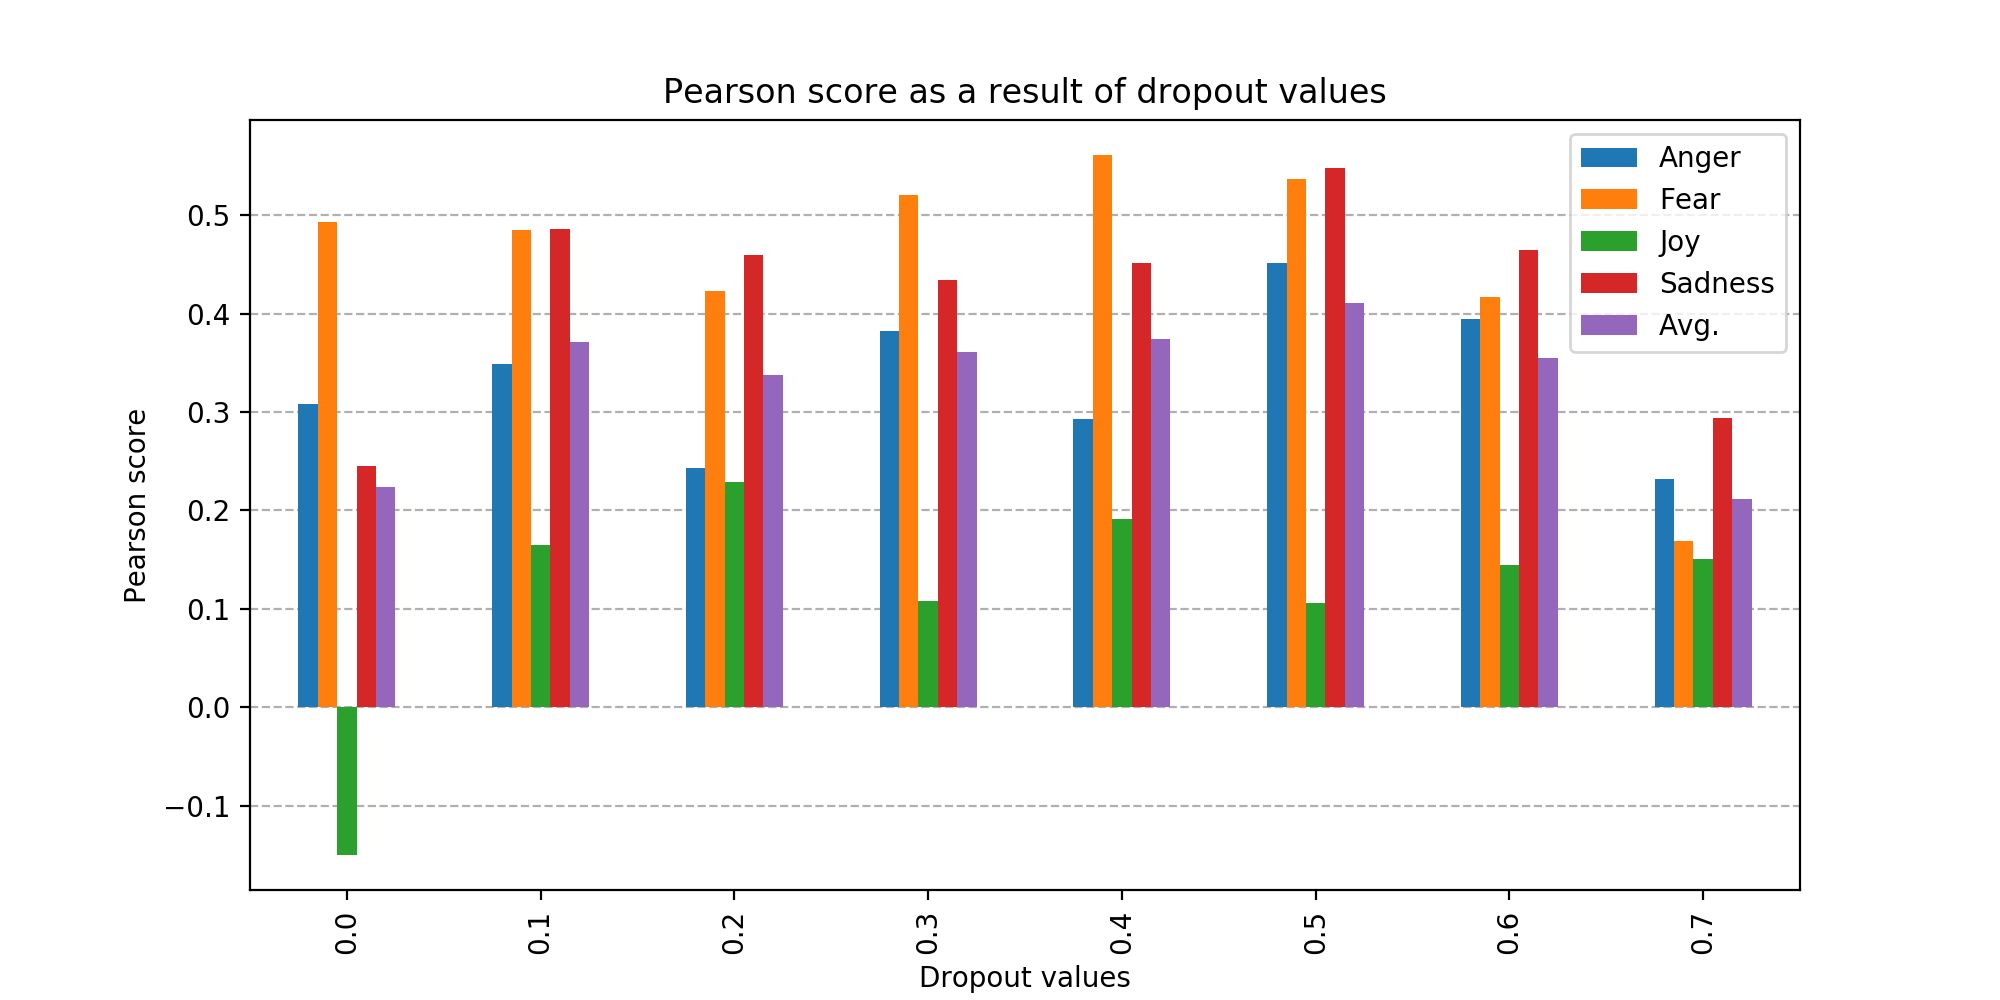
\includegraphics[width=\textwidth]{pictures/dropoutvalues.png}
        \caption{Pearson scores as a function of dropout value, loss weight set to 0.45, weighted BCE set to 0.5}
        \label{fig:dropoutvalues}
\end{figure}

\begin{figure}[H]
    \centering
        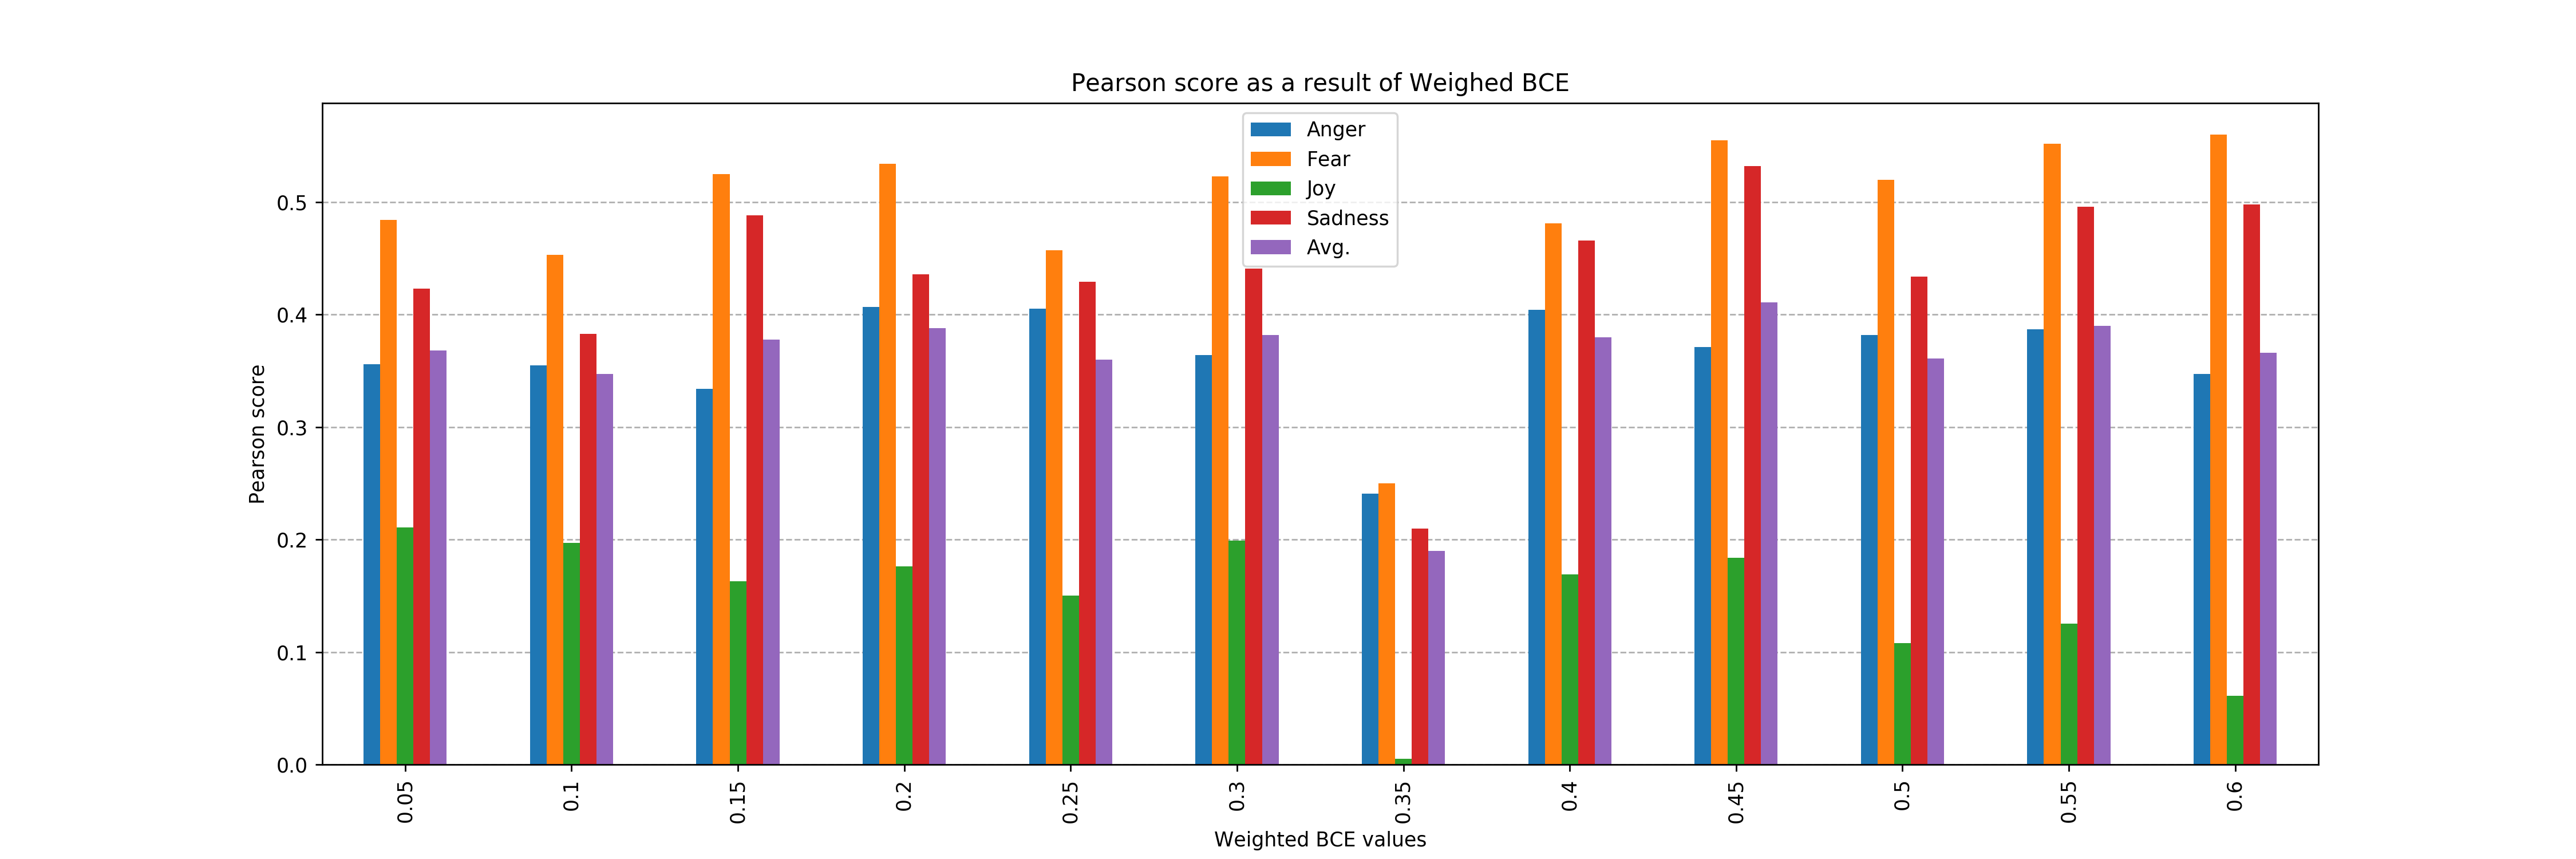
\includegraphics[width=\textwidth]{pictures/weightedBCEvalues.png}
        \caption{Pearson scores as a function of weighted BCE value, dropout set to 0.3, loss weight set to 0.45}
        \label{fig:BCEvalues}
\end{figure}

\begin{figure}[H]
    \centering
        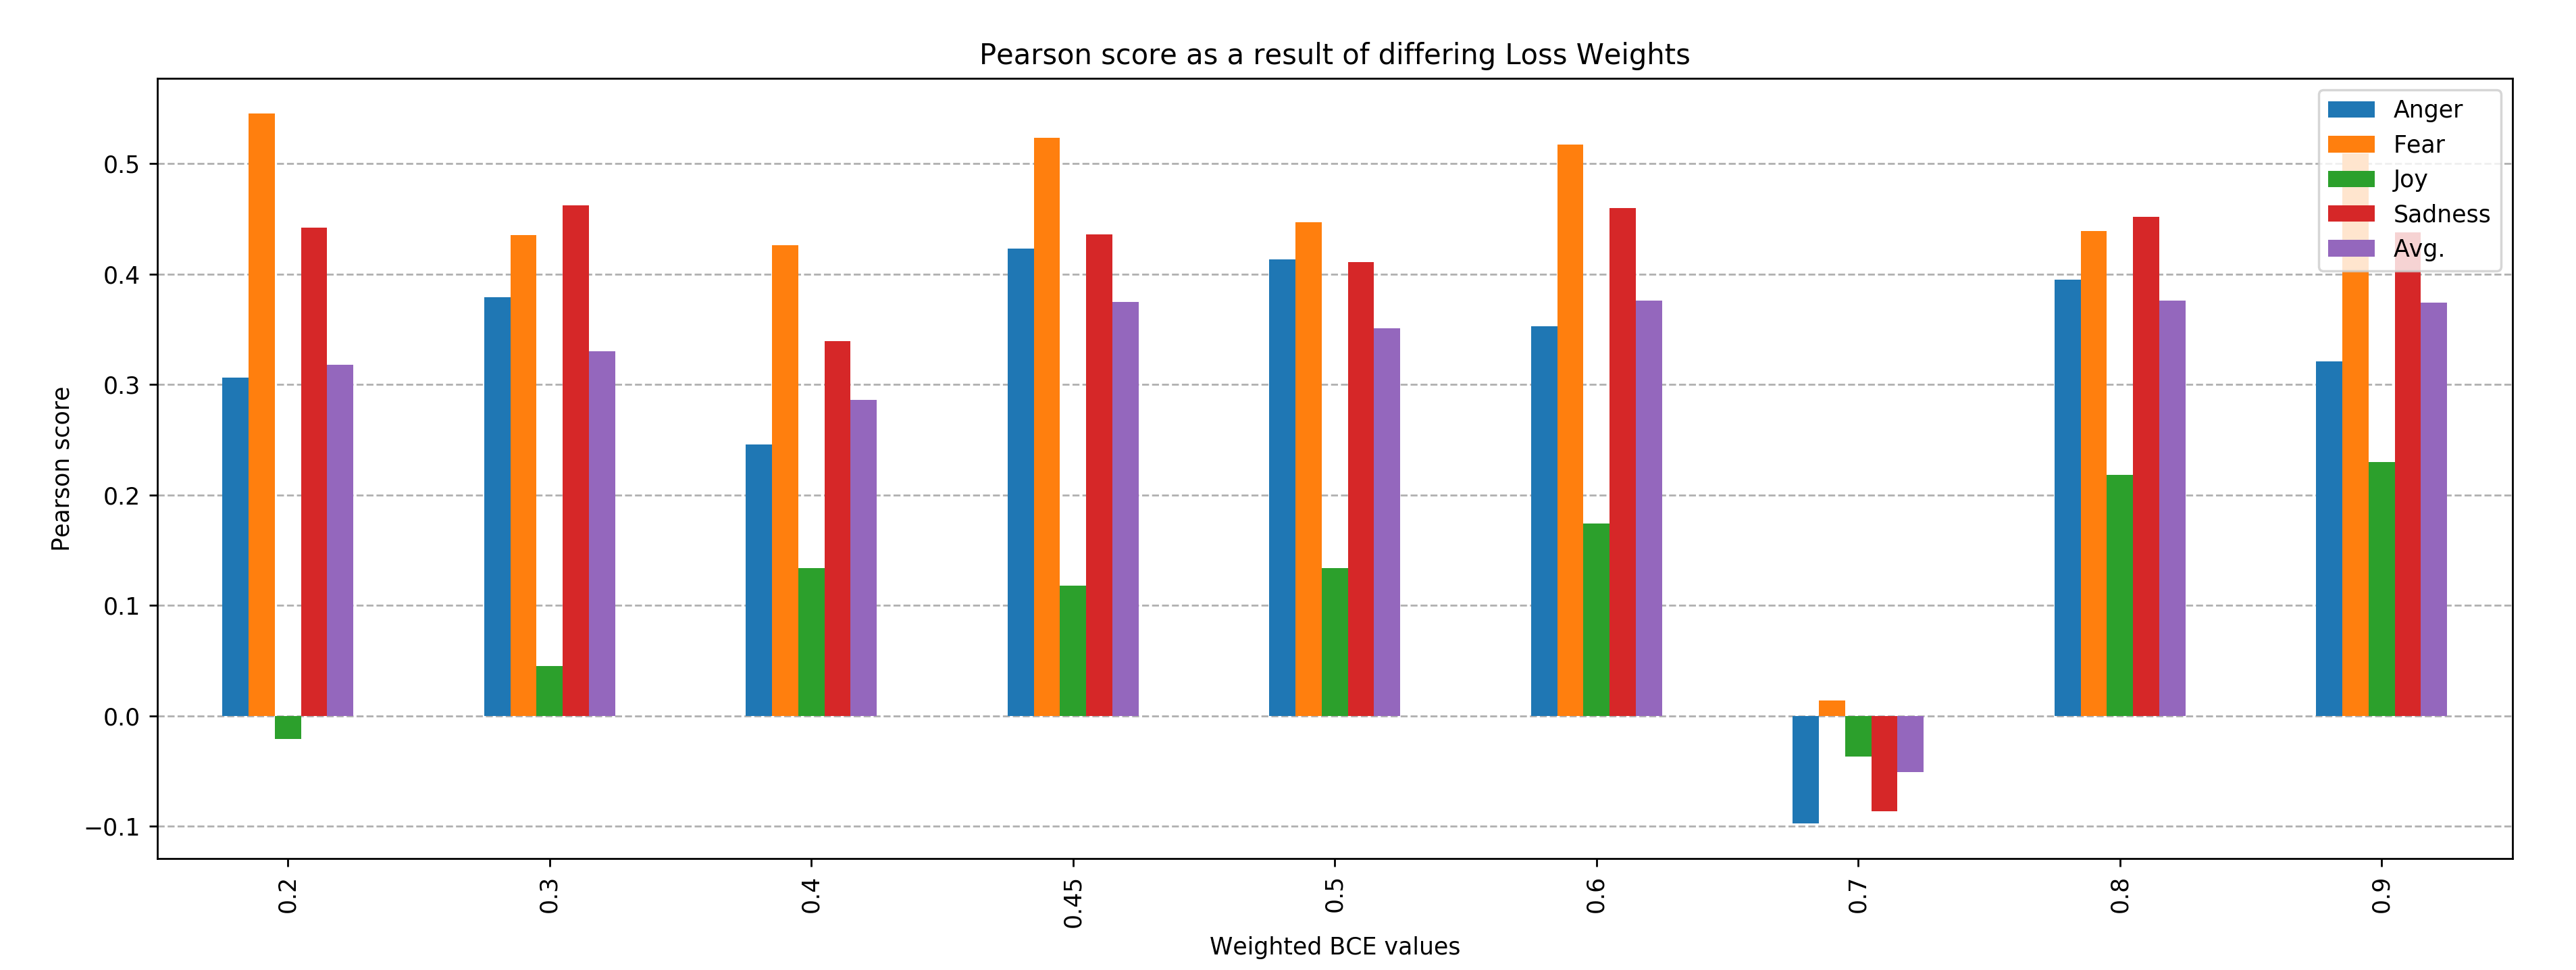
\includegraphics[width=\textwidth]{pictures/LossWeightsvalues.png}
        \caption{Pearson scores as a function of loss weight value, dropout set to 0.3, weighted BCE set to 0.45}
        \label{fig:LWvalues}
\end{figure}

\begin{figure}[H]
    \centering
        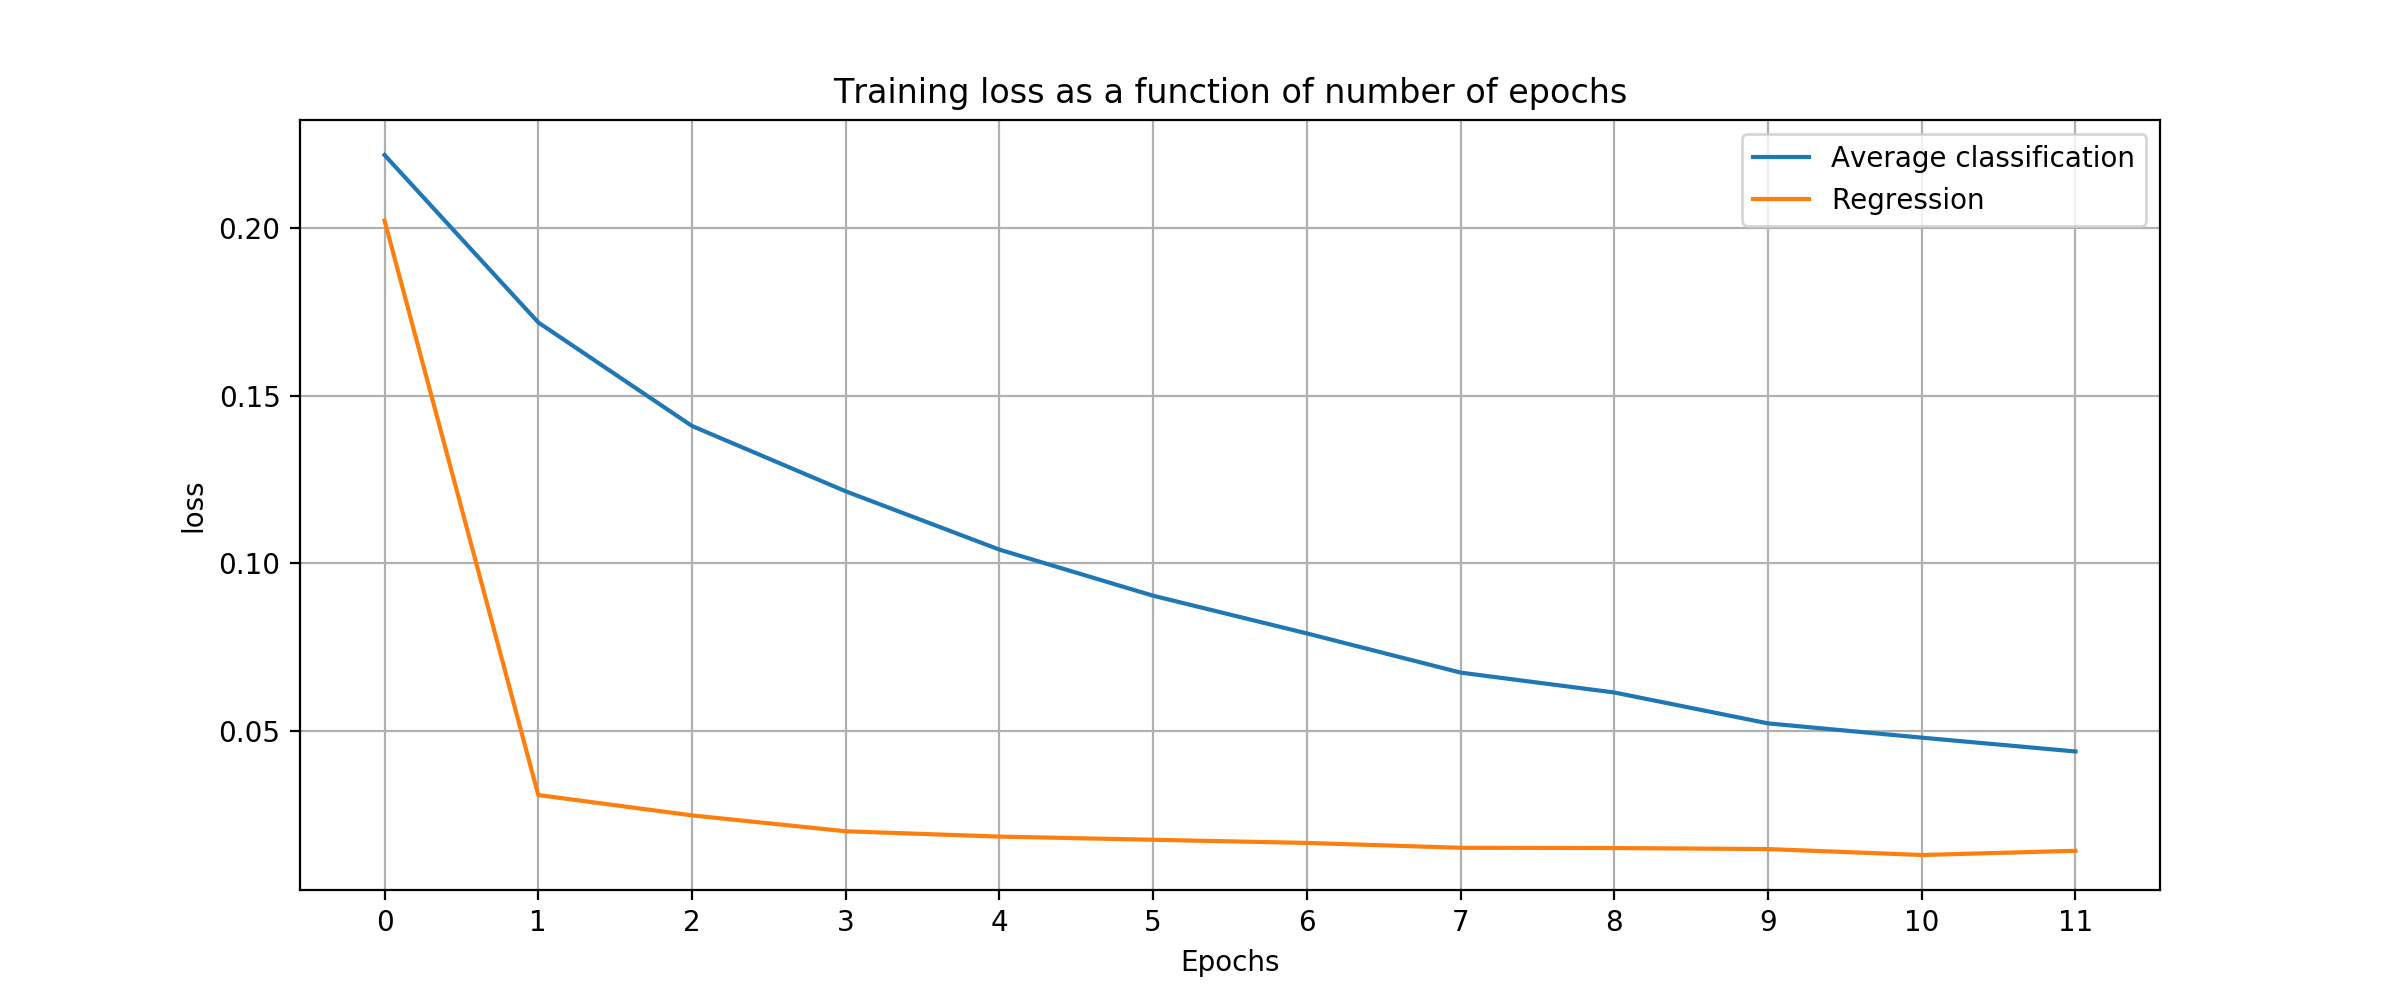
\includegraphics[width=\textwidth]{pictures/regclasstraining.png}
        \caption{Training loss as a function of epochs, dropout set to 0.3, weighted BCE set to 0.45}
        \label{fig:trainingloss}
\end{figure}

\begin{figure}[H]
    \centering
        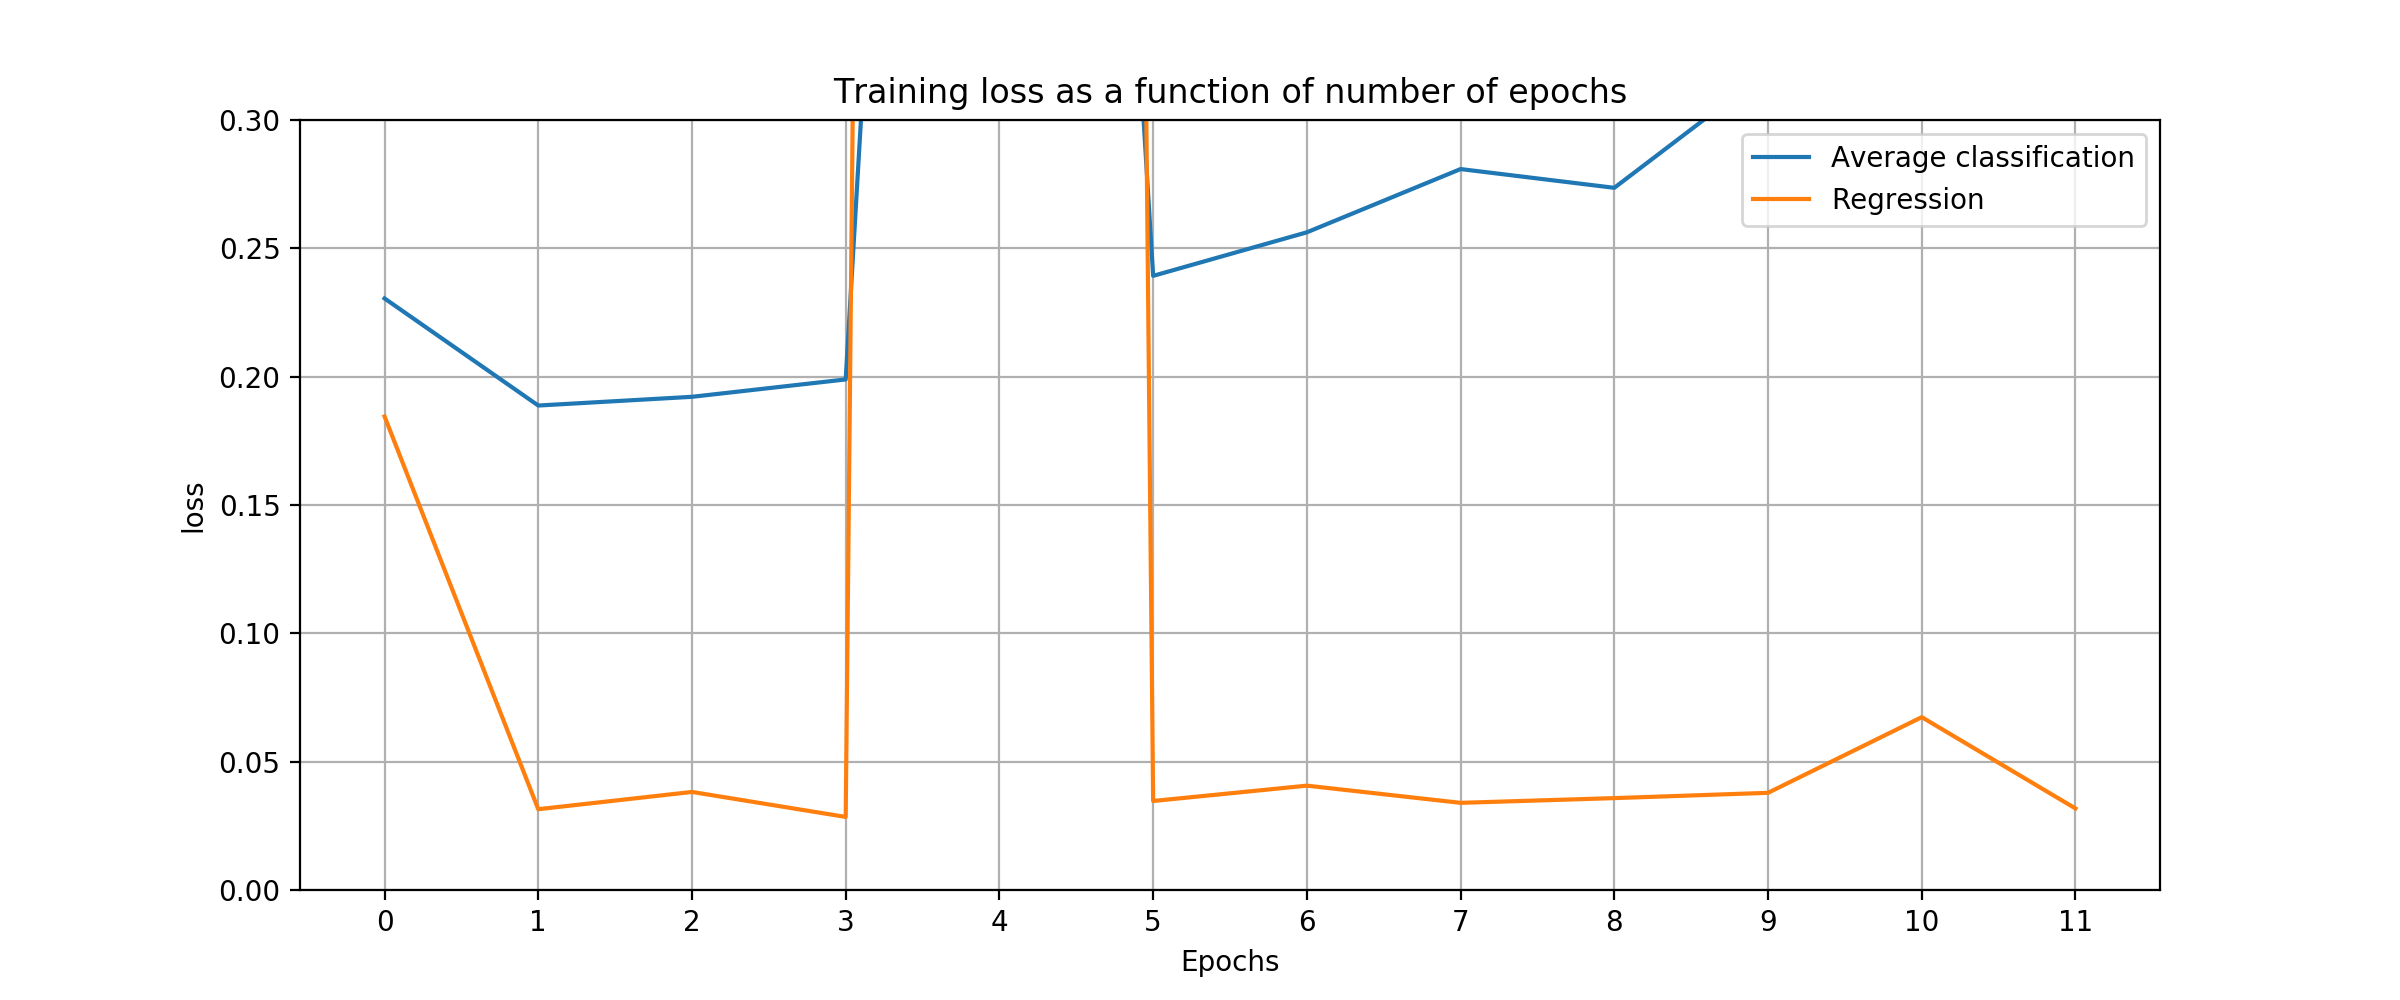
\includegraphics[width=\textwidth]{pictures/regclassvalidation.png}
        \caption{Validation loss as a function of epochs, dropout set to 0.3, weighted BCE set to 0.45}
        \label{fig:valloss}
\end{figure}


\bibliography{biblio}

\end{document}
